\chapter{State-of-art} \label{chap:sota}
% inference optimization
\section{CNN optimizations for FPGA} \label{sec:opti_cnn}
%
%
The previous chapter has described the way \acrshort{cnn} work and the different state-of-the-art models. Section \ref{subs:mbv2} evidenced the issue to implement the inference phase on mobile devices such as \acrshort{fpga}. Indeed, the computational complexity and the storage requirements are way beyond their capabilities. This section explores the state-of-the-art approaches to reduce the arithmetic complexity and the hardware utilization to handle this problem on a \acrshort{fpga}. First, Section \ref{subsec:algopti} details how to efficiently handle and optimize the convolution operation on \acrshort{fpga}. Then, Section \ref{subsec:mdopti} covers techniques to reduce the size of the model.
%
\section{Algorithmic Optimizations} \label{sec:algopti}
In this section we will review algorithmic optimization techniques to reduce computational complexity of convolutions, which are a costly operation. According to \cite{shawahna_fpga-based_2019}, 90\% of computation time in \acrshort{cnn} are consummed by the convolution operation.
%
%
\subsection{\acrfull{gemm}}
%
%
It is a common way to process \acrshort{cnn} on \acrshort{cpu} and \acrshort{gpu}. We convert the convolution as a matrix-vector multiplication.  The process of a convolution layer can be observed on Figure \ref{fig:gemm}.
However, this approach is not suggested for \acrshort{fpga}: \cite{sze_efficient_2017, zhu_efficient_2020} point out that the \acrshort{fm}s have to be copied multiple times when flattened to a vector. It leads to a huge memory footprint and either ineffiency in storage or complex memory management access patterns.
\begin{figure}
    \centering
    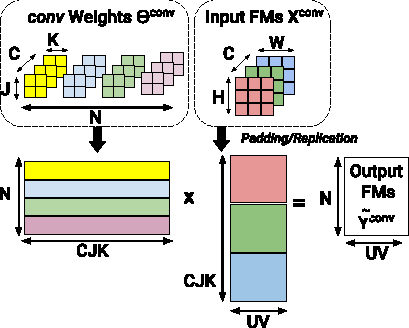
\includegraphics[width=0.5\textwidth]{Images/gemm.pdf}
    \caption{\acrshort{gemm} base processing on conv layer}
    \label{fig:gemm}
\end{figure}
%
%
\subsection{Winograd Transform}
%
%
The Winograd minimal filter algorithm is first introduced by \cite{winograd_arithmetic_1980}. We can apply this computational transform to convolutions when the stride is equal to 1. In Winograd filtering, data is processed by blocs referred as \textit{tiles}, as following:
\begin{itemize}
    \item An input \acrshort{fm} tile $g$ of size $(N_{ix} \times N_{iy})$ is pre-processed: $\tilde{g} = \boldsymbol{G^{T}} g \boldsymbol{G} $, where $\boldsymbol{G}$ is a transformation matrix defined in the Winograd Algorithm \cite{winograd_arithmetic_1980}.
    \item In a same way, $d$, the filter of size $(K_x \times K_y)$ is transformed into $\tilde{d}$: $\tilde{d} = \boldsymbol{B^{T}} d \boldsymbol{B}$ , where $\boldsymbol{B}$ is a transformation matrix defined in the Winograd Algorithm \cite{winograd_arithmetic_1980}.
    \item The output tile $Y$ of the Winograd Filtering algorithm, denoted $F(N_{ix} \times N_{iy}, K_x \times K_y)$ is computed using equation \ref{eqn:winograd}, where $\boldsymbol{A}$ is a transformation matrix defined in the Winograd Algorithm \cite{winograd_arithmetic_1980} and $\odot$ indicates element-wise multiplication.
\end{itemize}
\begin{equation}
\label{eqn:winograd}
Y = \boldsymbol{A^{T}} [ \ \tilde{g} \odot \tilde{d} \ ] \boldsymbol{A}
\end{equation}
\cite{lavin_fast_2015} demonstrated that Winograd convolution is efficient when the kernel is small ($K_* \leq 3$) and the number of multiplication can be reduced by a factor of $2.25 \times$ (in returns the number of addition is increased). According to \cite{sandler_mobilenetv2_2019}, $3 \times 3$ kernel is a standard for modern networks, which leads to think that Winograd Transform is a usefull approach to reduce computational complexity of convolutional layers. For example, \cite{aydonat_opencl_2017, lu_evaluating_2017} utilized Winograd transform and haved reduced their computational complexity by around 50\%.
%
%
\subsection{\acrfull{fft}}
%
%
The \acrshort{fft} is an algorithm to transform the 2D convolution into element-wise multiplication in the frequency domain. The equation is observed at equation \ref{eqn:fft}
\begin{equation}
\label{eqn:fft}
conv2D(FM_{I}[ic], K[oc, ic]) = IFFT( FFT(FM_{I}[ic]) \odot FFT(K[oc, ic]) )
\end{equation}
The arithmetic complexity of the 2D convolution can be reduced to $O(N_{ix}^2 log_2(N_{ix}))$ \cite{jong_hwan_ko_design_2017} and the computational complexity of the \acrshort{fft} can be reduced to $O(N_{ix} log_2(K_{x}))$ using the Overlap-and-Add Method \cite{w_smith_scientist_1997}.
However, the \acrshort{fft} finds its interest when kernel are large \cite{lavin_fast_2015} ($K_* \geq 5$), which is not a standard kernel size according to \cite{sandler_mobilenetv2_2019}. \cite{zhang_frequency_2017} implemented \acrshort{fft} algorithm for \acrshort{cnn} on \acrshort{fpga} and it showed little reduction of computation complexity with small filters such as $3 \times 3$.

%
\subsection{Model Optimizations} \label{subsec:mdopti}
As mentioned previously, the major issues, when implementing a \acrshort{cnn} on an \acrshort{fpga}, are the \acrshort{cnn} size and its computational complexity. Research was done to develop techniques tackling those two issues by directly modifying the \acrshort{cnn} architecture. \textcite{nurvitadhi_can_2017} believe that sparsity exploitation and extremely compact data types will become the norm in next-generation \acrshort{cnn}s.
%
%
\subsubsection{Efficient Model Design}
%
Section \ref{subsec:models} presented several state-of-the-art models. However, those models (except MobileNetV2) were designed to provide the highest performance possible but did not consider the implementation of such models on mobile and embedded devices \cite{iandola_squeezenet_2016}. Therefore, several other models were designed to run on such constrained platforms trading a reduction of the number of parameters and operations in exchange for a drop of accuracy. Indeed, if we observe Figure \ref{fig:archi}, the lightweight models do not match the high-performance ones in terms of accuracy only.

A clever choice of design decreases the number of parameters and computations of the model while reducing the drop of accuracy. As many approaches were proposed to reduce the size of a model, this study will focus on architectures that target the embedded space. This section describes five of these architectures:
\begin{itemize}
    \item \textbf{SqueezeNet} \cite{iandola_squeezenet_2016} was focused on reducing the number of parameters of AlexNet (see Section \ref{subsec:models}) by introducing a new building block: \textbf{Fire Module}. Therefore, their architectures are very similar. SqueezeNet replaces all layers (except the first and last one) by \textbf{Fire Modules}. The \textbf{Fire Module}, observed in Figure \ref{fig:archi_building_block:sqn}, is composed of two convolutional layers. The first one called \textit{squeeze block} only performs $1 \times 1$ convolutions to squeeze the number of input channels. The reduction of the number of channels decreases the computational complexity and number of parameters of the next convolutional layer. Moreover, they also chose $1 \times 1$ convolution because it requires fewer parameters than $3 \times 3$ convolution.
    The second convolutional layer called \textit{expand block} is composed of $1 \times 1$ and $3 \times 3$ convolutions. With this architecture, the size of AlexNet is decreased from $240$MB to $4.8$MB \cite{iandola_squeezenet_2016}. It can even be reduced to $0.47$MB without a drop in accuracy method by applying Deep Compression \cite{han_deep_2016}. However, it has a big memory footprint, is slower in runtime, and consumes more energy than AlexNet \cite{sze_efficient_2017}.
    %
    \item \textbf{MobileNet} \cite{howard_mobilenets_2017} uses \acrshort{dsc}, described in Section \ref{subs:dsc}, to build small and low latency models that can fulfill the design requirements, as can be seen in Figure \ref{fig:archi_building_block:mbn}. Two hyper-parameters are used to set the model size and throughput:
    %
    \begin{itemize}
        \item The width multiplier $\alpha \in [1; 0[$, which reduces the number of input and output channels at each layer,
        \item The resolution multiplier $\rho \in [1; 0[$,  which reduces spatially the input and output \acrshort{fm}s at each layer.
    \end{itemize}
    %
    \item \textbf{ShuffleNet}  was developed by \textcite{zhang_shufflenet_2018}, in 2018. It is designed to be a computation efficient architecture, especially for mobile devices with very limited computing power. Indeed, it reduces the computation cost while maintaining the accuracy by using \textbf{pointwise group convolution}, decreasing the computation complexity of $1 \times 1$ convolutions. It also uses \textbf{channel shuffle} operation on the channels such that \textbf{group convolutions} obtain information from different groups. Then more powerful structures can be built with multiple group convolutional layers. However, the group convolutions and the bottleneck structures add \acrfull{mac} which is a non-negligible cost \cite{ma_shufflenet_2018}. The group convolution contributes to network fragmentation and reduces parallelism. Moreover, the \textquote{Add} operation, as seen in Figure \ref{fig:archi_building_block:shn}, is quite significant.
    %,
    \item \textbf{NasNet} was developed by \textcite{zoph_learning_2018}, in 2018. The idea was to use a search method called \acrfull{nas}, to find good convolutional architectures on a specific dataset. For that purpose, NasNet uses a \acrfull{rnn} to generate efficient architectures. The \acrshort{rnn} generates sample child networks with different architectures, which are trained to convergence. The accuracy of the child networks is used to train the \acrshort{rnn}, which will generate better architectures over time. A convolution layer can be seen in Figure \ref{fig:archi_building_block:nasn}. The learned architecture is flexible as it may be scaled in terms of computational cost. The network provides a higher accuracy with comparable parameters and \acrshort{mac} than MobileNet and ShuffleNet (described previously) \cite{zoph_learning_2018}. However, the resulting network ends up very complex \cite{sandler_mobilenetv2_2018}.
    %
    \item \textbf{MobileNetV2} was developed by \textcite{sandler_mobilenetv2_2018}, in 2018. It is an improvement of MobileNet (described previously) in terms of accuracy and does not require special operators. It has also a smaller memory footprint. Furthermore, MobileNetV2 has faster inference and fewer parameters than MobileNet. MobileNetV2 has already been explained in Section \ref{subs:mbv2}.
\end{itemize}
%
\begin{figure}[H]
    \centering
    %
    \begin{subfigure}[t]{0.49\linewidth}
        \centering
        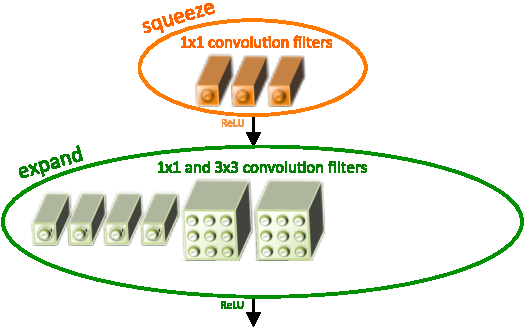
\includegraphics[width=\textwidth, height=0.3\textheight, keepaspectratio]{squeeze.pdf}
        \caption{Squeezenet Fire Module\cite{iandola_squeezenet_2016}}
        \label{fig:archi_building_block:sqn}
    \end{subfigure}
    %
    \begin{subfigure}[t]{0.49\linewidth}
        \centering
        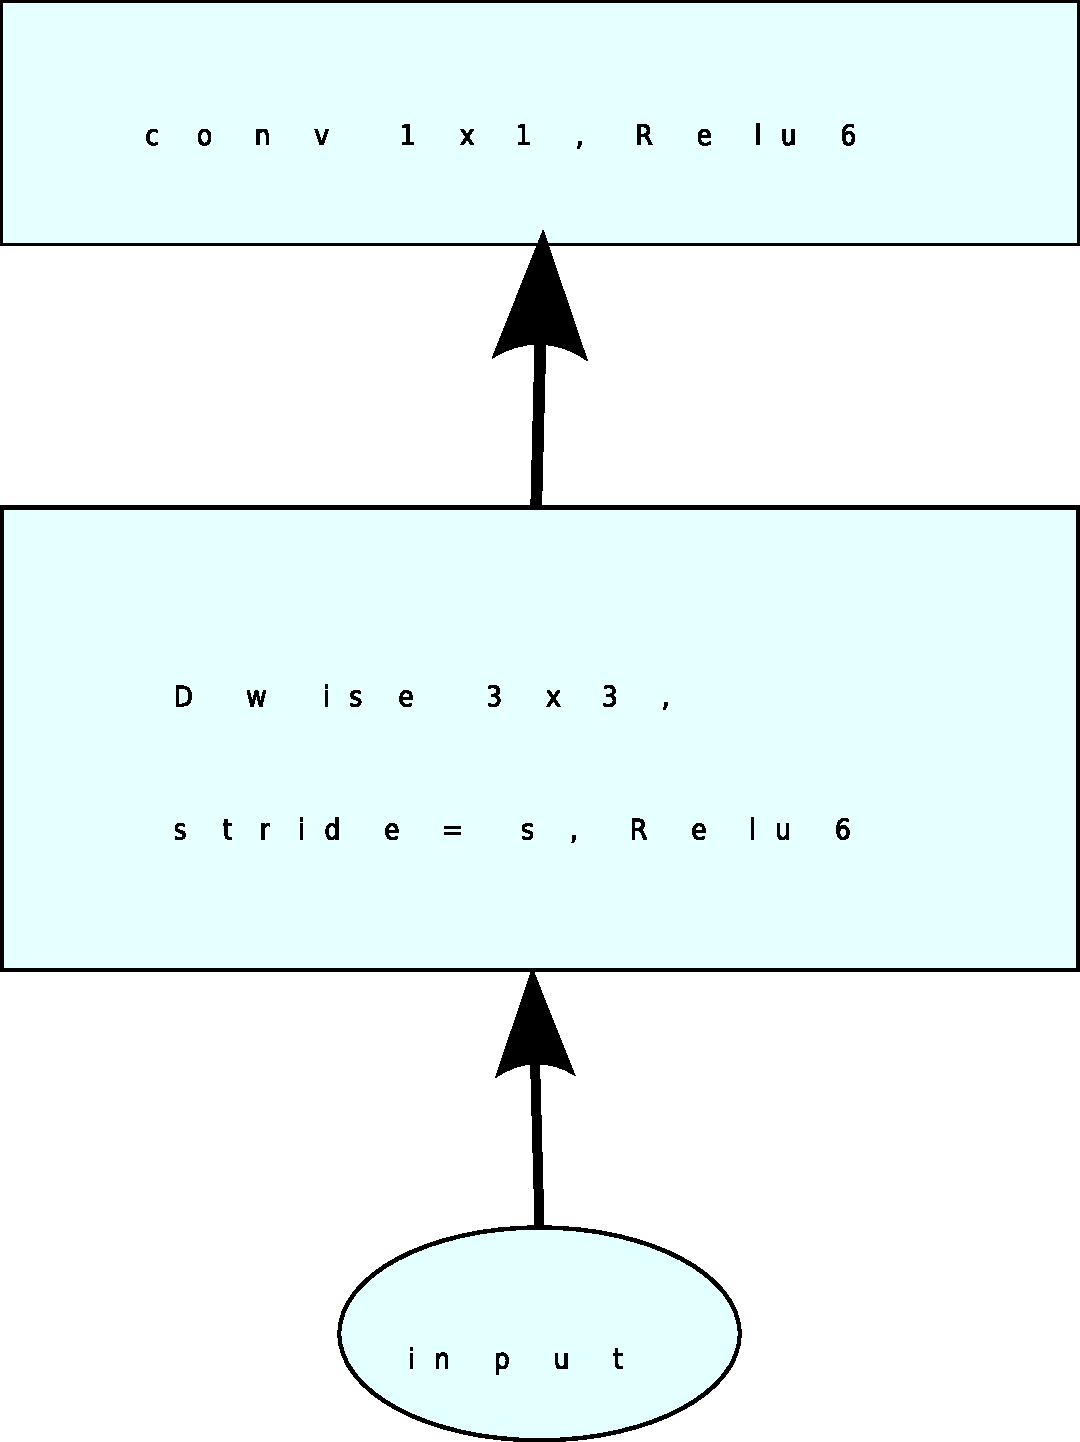
\includegraphics[width=\textwidth, height=0.2\textheight, keepaspectratio]{mobilenet.pdf}
        \caption{MobileNet convolutional block \cite{howard_mobilenets_2017}}
        \label{fig:archi_building_block:mbn}
    \end{subfigure}
    %
    \begin{subfigure}[t]{0.49\linewidth}
        \centering
        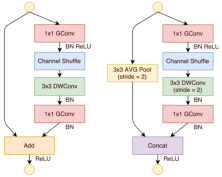
\includegraphics[width=\textwidth, height=0.2\textheight, keepaspectratio]{shufflenet.pdf}
        \caption{ShuffleNet convolutional block \cite{zhang_shufflenet_2018}}
        \label{fig:archi_building_block:shn}
    \end{subfigure}
    %
    \begin{subfigure}[t]{0.49\linewidth}
        \centering
        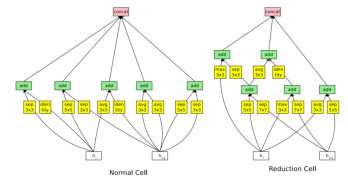
\includegraphics[width=\textwidth, height=0.3\textheight, keepaspectratio]{nasnet.pdf}
        \caption{NasNet convolutional blocks \cite{zoph_learning_2018}}
        \label{fig:archi_building_block:nasn}
    \end{subfigure}
    %
    \begin{subfigure}[t]{0.49\linewidth}
        \centering
        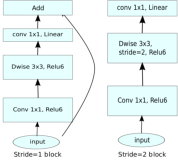
\includegraphics[width=\textwidth, height=0.2\textheight, keepaspectratio]{mobilenet2.pdf}
        \caption{MobileNetv2 convolutional blocks \cite{sandler_mobilenetv2_2018}}
        \label{fig:archi_building_block:mb2n}
    \end{subfigure}
    %
    \caption{Convolutional block from different architectures}
    \label{fig:archi_building_block}
\end{figure}

The architecture used in this work was developed to implement MobileNetV2 because of its simplicity and its state-of-the-art performance (see Table \ref{tab:mbv2}). Moreover, MobileNetV2 requires fewer parameters while providing state-of-the-art accuracy when comparing to the different architectures, as shown in Figure \ref{fig:archi}.
%
\begin{table}[H]
    \center
    \begin{tabular}{ | c | c | c c | c| }
        \hline \hline
        Network & Top 1 & Params & MAdds & CPU \\
        \hline \hline
        MobileNetV1 & 70.6 & 4.2M & 575M & 113ms \\
        ShuffleNet (1.5) & 71.5 & \textbf{3.4M} & 292M & - \\
        ShuffleNet (x2)  & 73.7 & 5.4M & 524M & - \\
        NasNet-A & 74.0 & 5.3M & 564M & 183ms \\
        \hline
        MobileNetV2 & \textbf{72.0} & \textbf{3.4M} & \textbf{300M} & \textbf{75ms} \\
        MobileNetV2 (1.4) & \textbf{74.7} & 6.9M & 585M & \textbf{143ms} \\
        \hline \hline
    \end{tabular}
    \caption{Performance on ImageNet, comparison for different networks \cite{sandler_mobilenetv2_2018}}
    \label{tab:mbv2}
\end{table}

\begin{figure}[H]
    \centering
    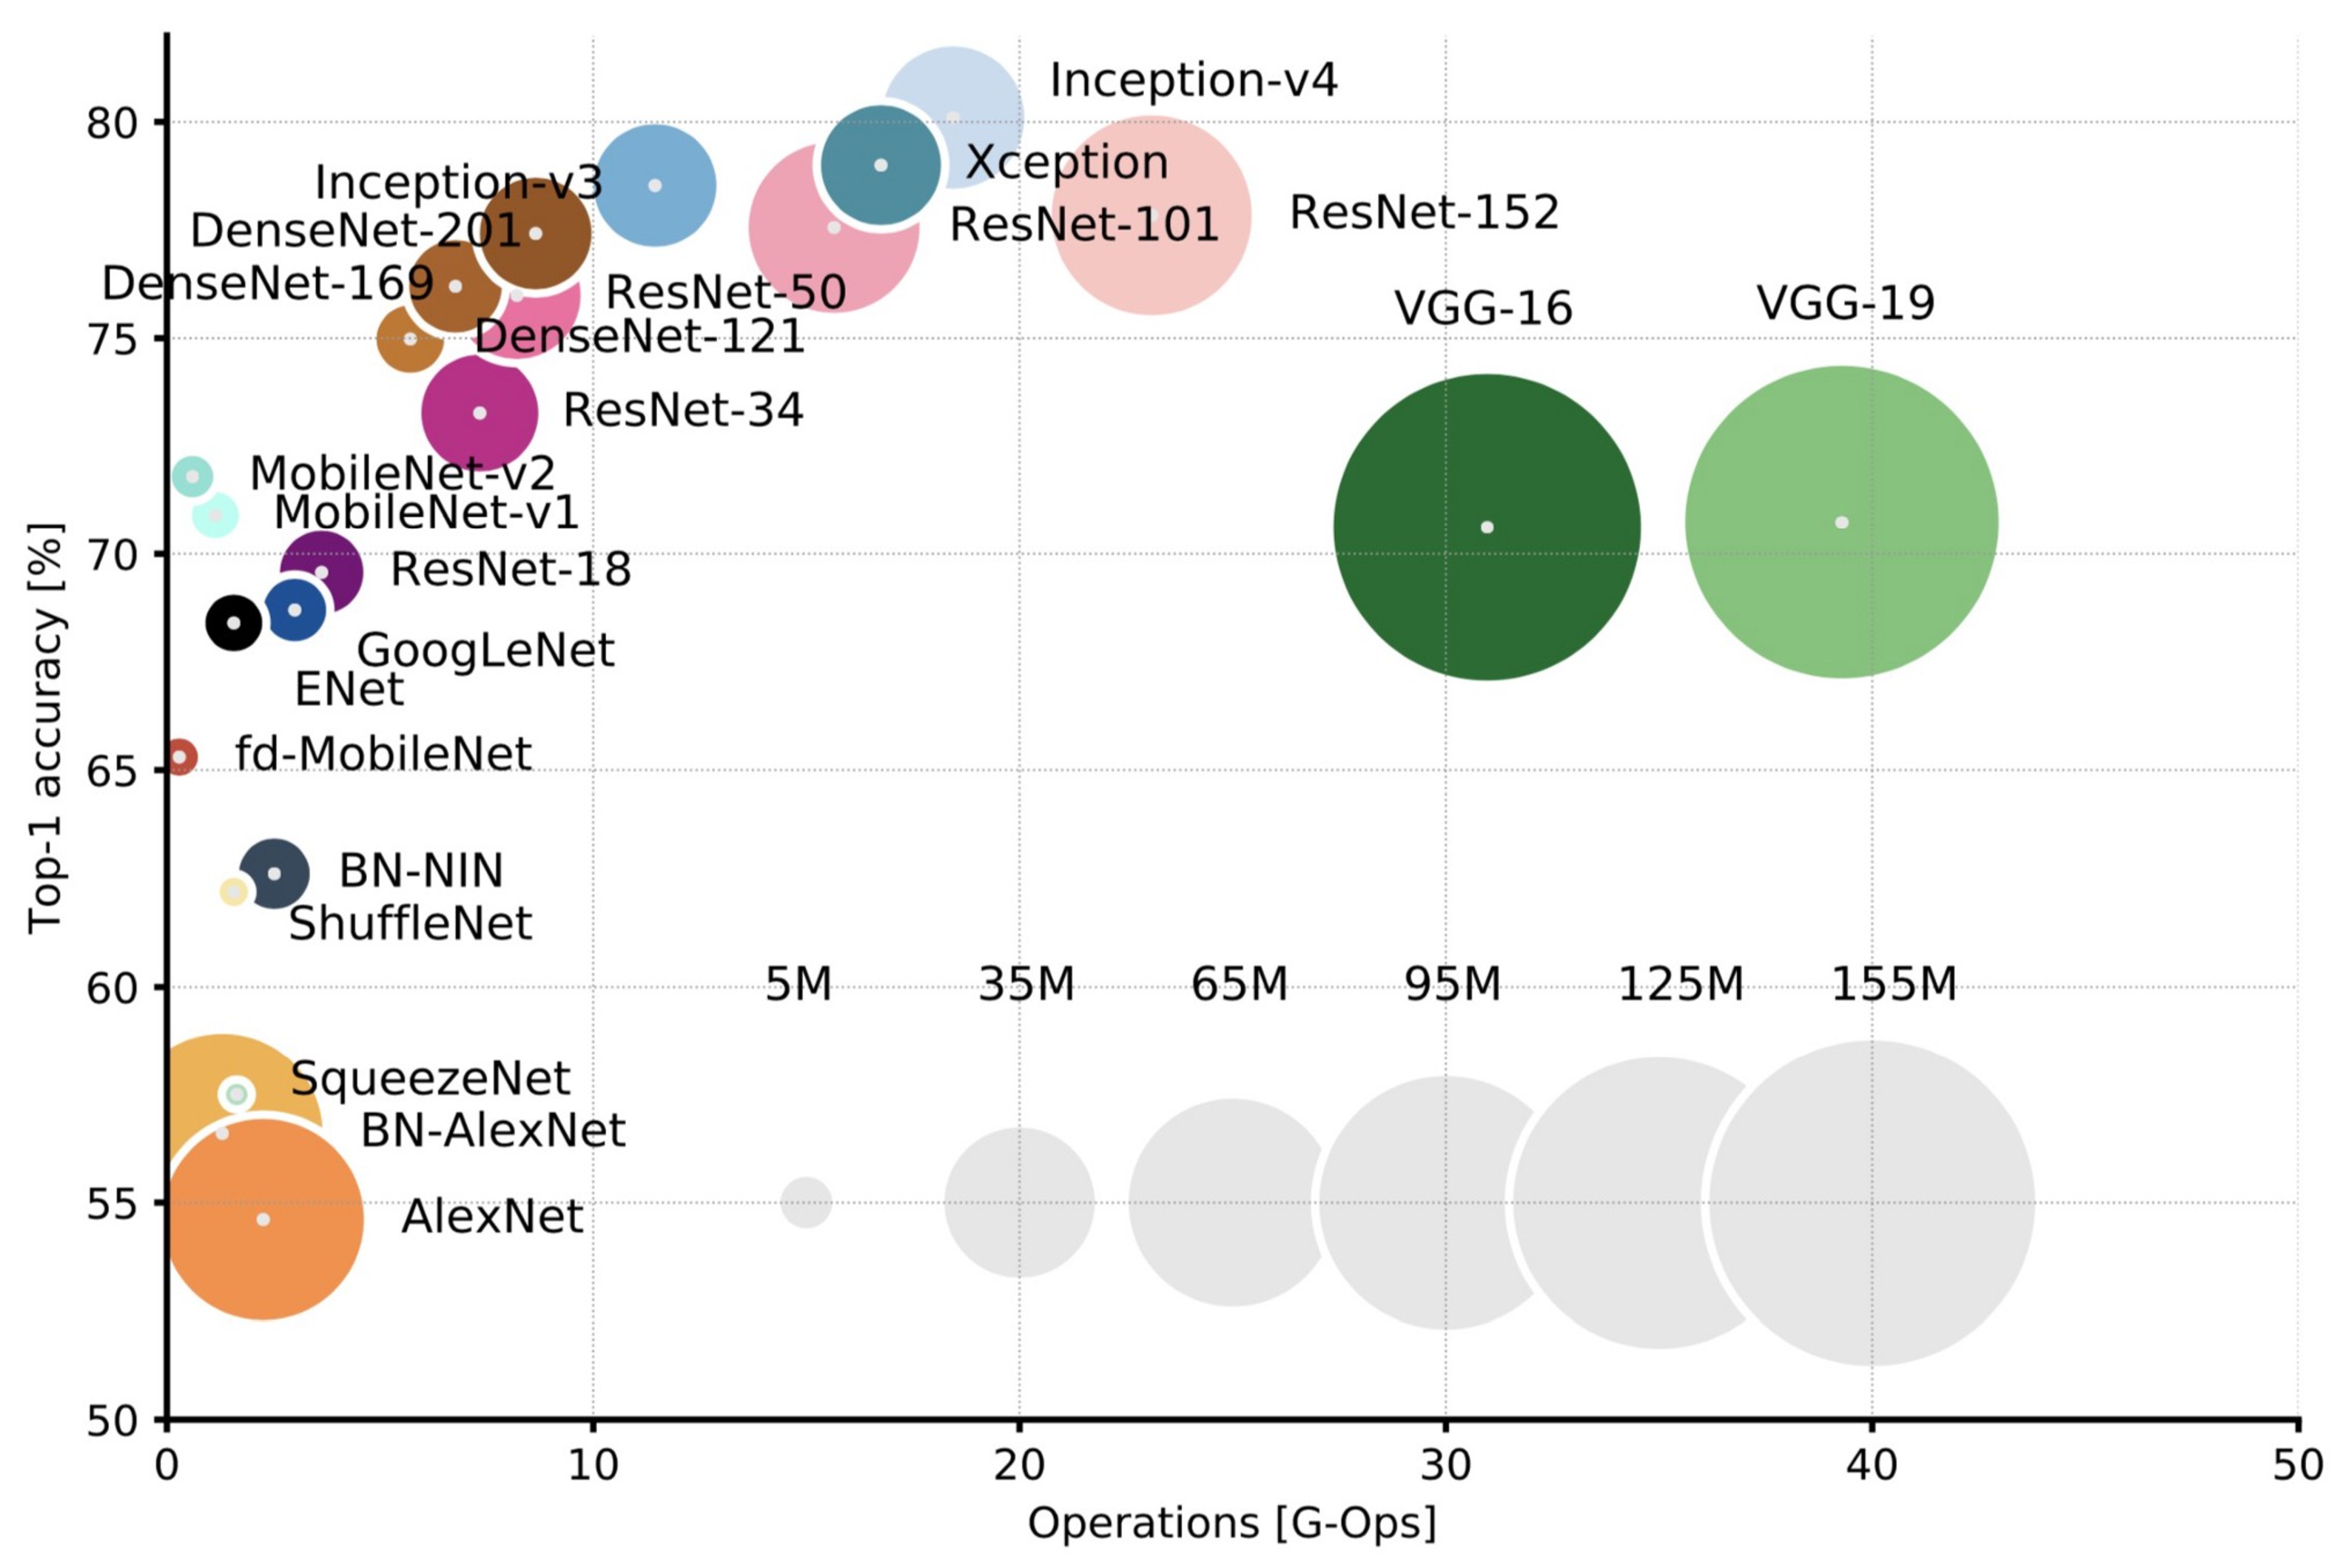
\includegraphics[width=0.9\textwidth]{archi.pdf}
    \caption{Ball chart reporting the Top-1 accuracy of various architectures vs. their computational complexity \cite{canziani_analysis_2017}}
    \label{fig:archi}
\end{figure}
%
\subsubsection{Pruning} \label{subs:pruning}
%
To improve the inference phase of a \acrshort{cnn}, pruning can be used, especially for platforms with limited computational resources \cite{liu_rethinking_2019}. According to \textcite{liu_rethinking_2019, denton_exploiting_2014}, the huge number of parameters in a network might create a problem of \textbf{over-parametrization}. Over-parametrization means that there are redundancies in \acrshort{nn} parameters and that the same performance could be achieved with only a subset of them. In other words, a lot of parameters are unimportant or unnecessary \cite{cheng_recent_2018}. Pruning is defined as removing the parameters considered as not important. For example, \textcite{baoyuan_liu_sparse_2015} achieve more than 90\% sparsity of parameters in convolutional layers in AlexNet with less than 1\% accuracy loss.

We can explain why pruning works by \textbf{The Lottery Ticket Hypothesis} \cite{frankle_lottery_2018, frankle_early_2020}: \textquote{\textit{A randomly initialized, dense neural network contains a subnetwork that is initialized such that—when trained in isolation—it can match the test accuracy of the original network after training for at most the same number of iterations.}} From this postulate, those unimportant weights can be set to zero (prune) because they do not improve the accuracy of the model.

According to \textcite{cheng_recent_2018}, pruning has two major benefits for the inference phase. First, less storage is required. Indeed, the non-pruned weights are sparsely distributed among the kernels. Thus, they can be stored in a compressed format reducing memory utilization. Second, pruning reduces the arithmetic complexity of the network. As convolutions perform a weighted sum with the input \acrshort{fm}, each \acrfull{mac} operation with a pruned weight can be discarded. Moreover, \textcite{han_learning_2015, mao_exploring_2017, kang_accelerator-aware_2020} pointed out that some pruning ratios can also improve the accuracy of the network, which can be explained by a form of regularization.

Various pruning schemes are focused on increasing the sparsity of the network without a drop of accuracy \cite{han_deep_2016, han_learning_2015}.  We call this pruning scheme where all unimportant parameters are pruned without extra constraint \textbf{unstructured pruning} \cite{cheng_recent_2018}. However, it is challenging to exploit the performance and the high parallelism of \acrshort{fpga} with this kind of pruned network. Indeed, this kind of pruning scheme creates irregularities in the data access pattern \cite{zhu_efficient_2020}. It means that the number of pruned weights is different in each kernel, and we should adapt the circuitry to the worst case. As a consequence, all filters conduct wasteful operations except the worst case \cite{shimoda_filter-wise_2019}. Furthermore, \textcite{anwar_structured_2017} pointed out that unstructured pruning requires overhead for computing addresses of the sparse non-pruned elements. Therefore, we should find pruning patterns that would be more hardware-friendly.

In contrast to the unstructured pruning, we have \textbf{structured pruning} schemes \cite{kang_accelerator-aware_2020}. They combine a structure regularization for accuracy and locality optimization for computation efficiency. According to \textcite{anwar_structured_2017}, \textquote{\textit{Structured pruning has no or little extra costs}}. We can categorize the various schemes into different groups \cite{cheng_recent_2018, kang_accelerator-aware_2020, anwar_structured_2017, wen_learning_2016}:
\begin{itemize}
    \item \textbf{Depth-wise}: all the weights of a layer are pruned. The layer is then removed.
    \item \textbf{Kernel-wise}: instead of pruning all the weights, we keep a ratio of kernels, which means a reduction of the number of output channels. This pruning scheme is provided in Figure \ref{fig:struct_pruning:fw}.
    \item \textbf{Channel-wise}: it is one of the most popular methods because it still can fit in the convolutional deep learning frameworks \cite{liu_rethinking_2019}. A layer of the input \acrshort{fm} is pruned, which means that the layer is also pruned in all the kernels, as can be seen in Figure \ref{fig:struct_pruning:chw}.
    \item \textbf{Shape-wise}: we prune the same weights in each kernel or group of kernels. For example, this pruning scheme was used in \textcite{zhu_efficient_2020}. It is illustrated in Figure \ref{fig:struct_pruning:sw}
\end{itemize}
%
\begin{figure}[H]
    \centering
    %
    \begin{subfigure}[t]{.32\textwidth}
    \centering
    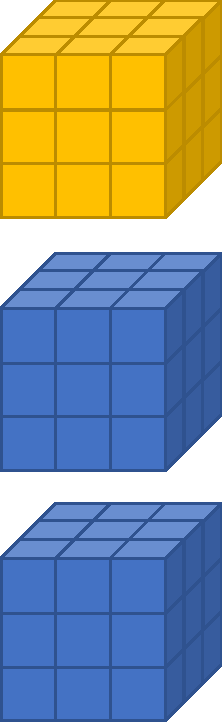
\includegraphics[width=0.33\linewidth]{filterwise.pdf}
    \caption{kernel-wise pruning}
    \label{fig:struct_pruning:fw}
    \end{subfigure}
    %
    \begin{subfigure}[t]{.32\textwidth}
    \centering
    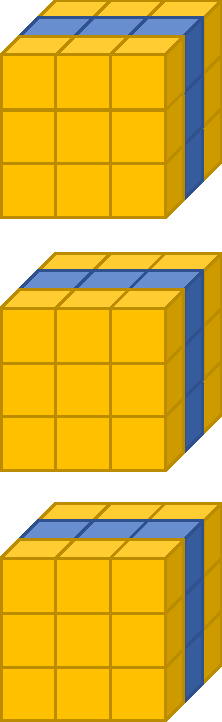
\includegraphics[width=0.33\linewidth]{channelwise.pdf}
    \caption{channel-wise pruning}
    \label{fig:struct_pruning:chw}
    \end{subfigure}
    %
    \begin{subfigure}[t]{.32\textwidth}
    \centering
    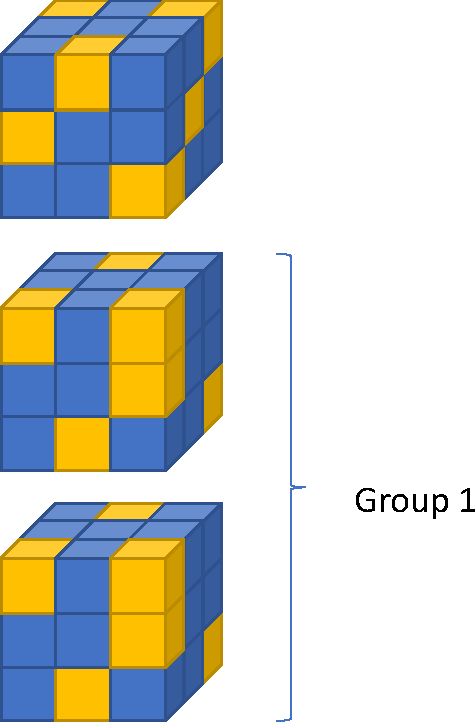
\includegraphics[width=0.70\linewidth]{shapewise.pdf}
    \caption{shape-wise pruning}
    \label{fig:struct_pruning:sw}
    \end{subfigure}
    %
    \caption{Structured pruning schemes, where the yellow weights are the pruned ones, inspired by \cite{cheng_recent_2018}}
    \label{fig:struct_pruning}
\end{figure}
%
The previously cited pruning schemes are ordered from very coarse-grained to fine-grained sparsity \cite{mao_exploring_2017}. As explained previously, coarse-grained sparsity (channel-wise and filter-wise pruning) provides a higher acceleration and can be used when implementing \acrshort{cnn} on \acrshort{gpu} or \acrshort{cpu} \cite{cheng_recent_2018, mao_exploring_2017}. However, finer-grained ones provide higher accuracy and as the sparsity increases, the accuracy is less affected, as can be seen in Figure \ref{fig:pruning-accuracy}. Therefore, this work focuses on developing customized hardware that can exploit a more fine-grained sparsity \cite{mao_exploring_2017} to provide a higher pruning while limiting the drop of accuracy.
%
\begin{figure}[H]
    \centering
    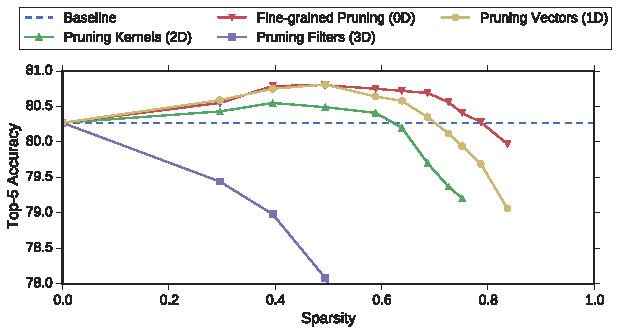
\includegraphics[width=\textwidth]{accuracysparsity.pdf}
    \caption{Accuracy-Sparsity Curve of AlexNet obtained by pruning \cite{mao_exploring_2017}}
    \label{fig:pruning-accuracy}
\end{figure}
%
Some studies focused on the acceleration of the inference step of lightweight models thanks to pruning. \textcite{zhang_channel_2019, tu_pruning_2019} applied pruning on \acrshort{dsc} kernels. They both chose \textbf{Channel-wise} pruning because it does not create sparse connections and it efficiently improves the speed of the inference. It also reduces the computational cost of the $1 \times 1$ (pointwise) convolutions, which has the biggest number of parameters and computational complexity. In MobileNet, it is about 95\%. By discarding one channel, the associated depthwise convolution is also avoided.
Moreover, the pointwise kernel producing that channel in the previous block can also be pruned. We can see the process in Figure \ref{fig:pruning_dsc}.
%
\begin{figure}[H]
    \centering
    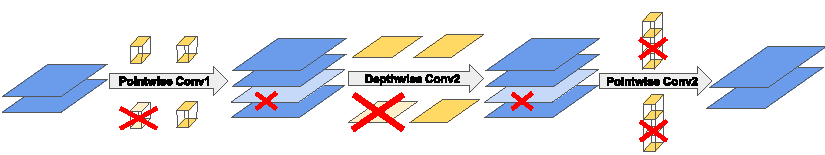
\includegraphics[width=\textwidth]{channelwise_ex.pdf}
    \caption{Pruning a depthwise separable convolution \cite{tu_pruning_2019}}
    \label{fig:pruning_dsc}
\end{figure}

\textbf{In this work, we focus on a structured pruning scheme for depthwise separable convolution. More precisely, we develop an architecture on \acrshort{fpga} than combines both advantages of pruning and depthwise separable convolution.}
%
\subsubsection{Quantization} \label{subs:quantization}
%
%
Quantization is an approach to trade accuracy for a decrease of the storage requirements of a network \cite{han_deep_2016}. Indeed, we can define quantization as the reduction of the number of bits representing a weight or pixel. Moreover, instead of using a floating-point number, we can use a \textbf{fixed-point number} \cite{cheng_recent_2018}. As said previously, fixed-point numbers are known to be more efficient on hardware such as \acrshort{fpga} because we can use integer arithmetic \cite{david_hardware_2007}. Quantization to fixed-point numbers can then reduce the memory requirement and the latency of the inference stage.

The format to encode the fixed-point representation of a real number is the \textit{Q-format} \cite{ward_real-time_2001}. A N-bit number, noted $Q_{m.n}$, is divided into two parts separated by an implied binary point. The $m$ bits are used to represent the integer part of the number (including the sign bit), and the $n$ bits are used to represent the fractional part, as can be seen in Figure \ref{fig:Qformat}. The bitwidth associated with each part can be either the same, either fine-tuned for each layer after analysis. Indeed, \textcite{qiu_going_2016, yin_high_2018} choose a different range for each layer, but doing it for every weight is not memory-efficient.
%
\begin{figure}[H]
    \centering
    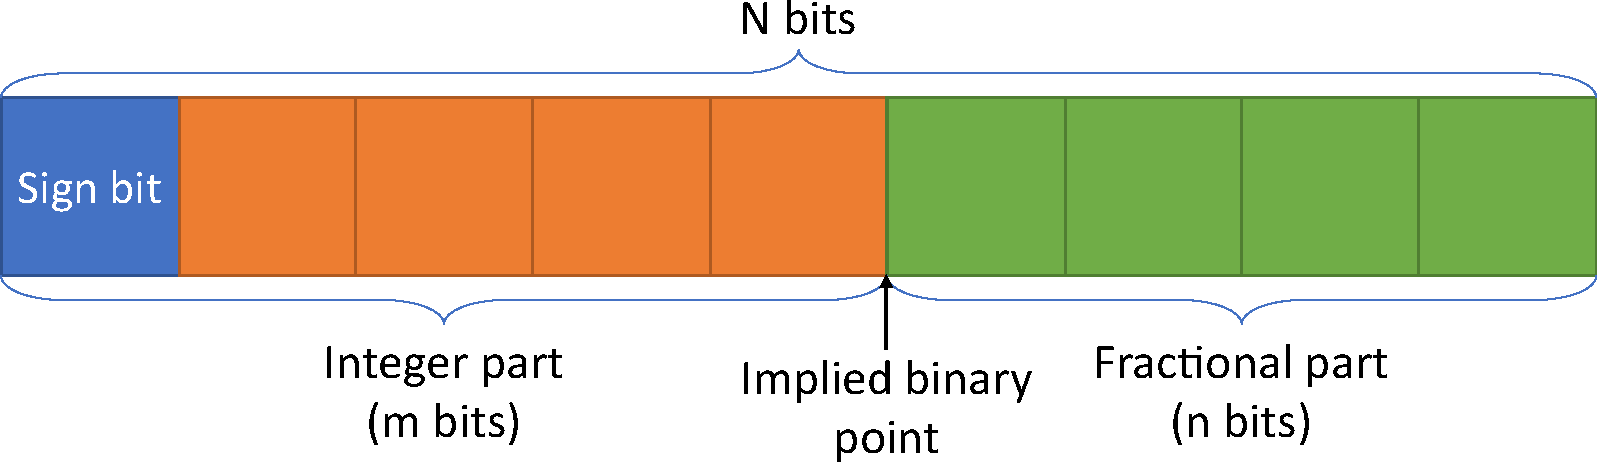
\includegraphics[width=\textwidth]{Qformat.pdf}
    \caption{Illustration of the Q-format}
    \label{fig:Qformat}
\end{figure}

As pointed out by \textcite{han_deep_2016}, quantization and pruning techniques are orthogonal and can be combined to compress further the network. Unfortunately, not all existing networks are friendly for quantization, like MobileNet. MobiletNet with quantized pixels and weights has a large drop of accuracy compared with its Non-quantized version (70.50\% using floating-point model vs 1.80\% using an 8-bit pipeline) \cite{sheng_quantization-friendly_2018}. However, the work of \textcite{sheng_quantization-friendly_2018} showed that the source of the accuracy drop was the design of the separable convolution core layer. They proposed therefore a new quantization-friendly separable convolution core layer. Works on MobileNetV2 should then be done to verify the fixed-point inference accuracy. Still, an 8-bit pipeline might not be optimal for MobilNetV2 as increasing the bitwidth to 16-bit could boost accuracy \cite{cheng_recent_2018}. This bitwidth is also widely used \cite{huimin_li_high_2016, bai_cnn_2018}. 

\textbf{Therefore, 16-bit fixed-point Q-format is adopted for input data, weights, and intermediate data in the frame of this thesis}. \textbf{Moreover, as said previously in Section \ref{subs:acti}, we can limit the integer part to 3 bits (one bit is added to express the sign of the weights), and we can use $Q_{4.12}$.}


%
\chapter{Accelerating \acrshort{cnn} inference on \acrshort{fpga}}
\label{chap:inf}
As said at chapter \ref{chap:intr}, interest has been made on accelerating the inference phase on \acrshort{fpga}. This chapter reviews the acceleration approaches to perform an efficient inference. \newline \newline
The three main optimization can be categorized according to \cite{abdelouahab_accelerating_2018}:
\begin{itemize}
    \item \textbf{Algorithmic Optimizations}: the computational cost of the convolution can be reduced by vectorizing them. More details can be found in section \ref{sec:algopti}.
    \item \textbf{Datapath Optimization}: because of the limited resources on a \acrshort{fpga}, memory if often the bottleneck and optimizing the memory management can increase the throughput. More details can be found in section \ref{sec:dtptopti}.
    \item \textbf{\acrshort{cnn} model Optimization}: an important issue of \acrshort{cnn} is their computational complexity and their hardware utilization. A solution is then to use approximate computing and trade accury for acceleration. This work focus on this kind of optimization. More details can be found in section \ref{sec:mdopti}.
\end{itemize}
%%%%%%%%%%%%
\section{Algorithmic Optimizations} \label{sec:algopti}
In this section we will review algorithmic optimization techniques to reduce computational complexity of convolutions, which are a costly operation. According to \cite{shawahna_fpga-based_2019}, 90\% of computation time in \acrshort{cnn} are consummed by the convolution operation.
%
%
\subsection{\acrfull{gemm}}
%
%
It is a common way to process \acrshort{cnn} on \acrshort{cpu} and \acrshort{gpu}. We convert the convolution as a matrix-vector multiplication.  The process of a convolution layer can be observed on Figure \ref{fig:gemm}.
However, this approach is not suggested for \acrshort{fpga}: \cite{sze_efficient_2017, zhu_efficient_2020} point out that the \acrshort{fm}s have to be copied multiple times when flattened to a vector. It leads to a huge memory footprint and either ineffiency in storage or complex memory management access patterns.
\begin{figure}
    \centering
    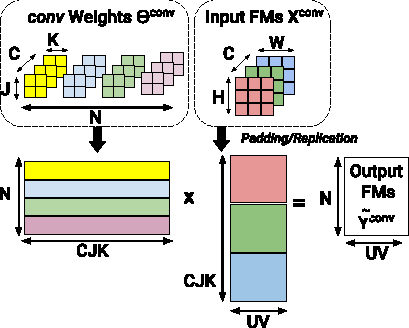
\includegraphics[width=0.5\textwidth]{Images/gemm.pdf}
    \caption{\acrshort{gemm} base processing on conv layer}
    \label{fig:gemm}
\end{figure}
%
%
\subsection{Winograd Transform}
%
%
The Winograd minimal filter algorithm is first introduced by \cite{winograd_arithmetic_1980}. We can apply this computational transform to convolutions when the stride is equal to 1. In Winograd filtering, data is processed by blocs referred as \textit{tiles}, as following:
\begin{itemize}
    \item An input \acrshort{fm} tile $g$ of size $(N_{ix} \times N_{iy})$ is pre-processed: $\tilde{g} = \boldsymbol{G^{T}} g \boldsymbol{G} $, where $\boldsymbol{G}$ is a transformation matrix defined in the Winograd Algorithm \cite{winograd_arithmetic_1980}.
    \item In a same way, $d$, the filter of size $(K_x \times K_y)$ is transformed into $\tilde{d}$: $\tilde{d} = \boldsymbol{B^{T}} d \boldsymbol{B}$ , where $\boldsymbol{B}$ is a transformation matrix defined in the Winograd Algorithm \cite{winograd_arithmetic_1980}.
    \item The output tile $Y$ of the Winograd Filtering algorithm, denoted $F(N_{ix} \times N_{iy}, K_x \times K_y)$ is computed using equation \ref{eqn:winograd}, where $\boldsymbol{A}$ is a transformation matrix defined in the Winograd Algorithm \cite{winograd_arithmetic_1980} and $\odot$ indicates element-wise multiplication.
\end{itemize}
\begin{equation}
\label{eqn:winograd}
Y = \boldsymbol{A^{T}} [ \ \tilde{g} \odot \tilde{d} \ ] \boldsymbol{A}
\end{equation}
\cite{lavin_fast_2015} demonstrated that Winograd convolution is efficient when the kernel is small ($K_* \leq 3$) and the number of multiplication can be reduced by a factor of $2.25 \times$ (in returns the number of addition is increased). According to \cite{sandler_mobilenetv2_2019}, $3 \times 3$ kernel is a standard for modern networks, which leads to think that Winograd Transform is a usefull approach to reduce computational complexity of convolutional layers. For example, \cite{aydonat_opencl_2017, lu_evaluating_2017} utilized Winograd transform and haved reduced their computational complexity by around 50\%.
%
%
\subsection{\acrfull{fft}}
%
%
The \acrshort{fft} is an algorithm to transform the 2D convolution into element-wise multiplication in the frequency domain. The equation is observed at equation \ref{eqn:fft}
\begin{equation}
\label{eqn:fft}
conv2D(FM_{I}[ic], K[oc, ic]) = IFFT( FFT(FM_{I}[ic]) \odot FFT(K[oc, ic]) )
\end{equation}
The arithmetic complexity of the 2D convolution can be reduced to $O(N_{ix}^2 log_2(N_{ix}))$ \cite{jong_hwan_ko_design_2017} and the computational complexity of the \acrshort{fft} can be reduced to $O(N_{ix} log_2(K_{x}))$ using the Overlap-and-Add Method \cite{w_smith_scientist_1997}.
However, the \acrshort{fft} finds its interest when kernel are large \cite{lavin_fast_2015} ($K_* \geq 5$), which is not a standard kernel size according to \cite{sandler_mobilenetv2_2019}. \cite{zhang_frequency_2017} implemented \acrshort{fft} algorithm for \acrshort{cnn} on \acrshort{fpga} and it showed little reduction of computation complexity with small filters such as $3 \times 3$.

%%%%%%%%%%%%
\subsection{General CNN inference on FPGA} \label{sec:dt_general}
%
As described in Section \ref{sec:fpga}, \acrshort{fpga} is an array of programmable gates that can interface with the outside world. As a result, to perform the convolution operation, the \acrshort{fpga} has to fetch weights and input \acrshort{fm} from the outside world (for example an external memory) and compute the convolution with them. Once the result is obtained, the \acrshort{fpga} can output the results through its \acrshort{ioe}.

According to \textcite{chen_eyeriss_2017}, the data movement can often be more energy-consuming than actual computation. Therefore, smart memory management is required to implement \acrshort{cnn} on low power devices such as \acrshort{fpga}. We discover in this section various techniques for handling the Datapath on the \acrshort{fpga}.

\subsubsection{Systolic Arrays}
%
%
Systolic arrays were implemented on the early \acrshort{fpga}-based accelerators \cite{abdelouahab_accelerating_2018, farabet_cnp_2009, gokhale_240_2014}. A static systolic array is a static array of \acrfull{pe}, controlled by the \acrshort{cpu}. The \acrshort{pe} is the basic computing unit for convolution. Therefore, each \acrshort{pe} is involved in a part of the computation and can communicate with adjacent \acrshort{pe}s. An illustration of this principle can be found in Figure \ref{fig:sytar}. The configuration can only support convolution with a kernel size $K_*$ lower than a maximal kernel size, such that $K_* \leq K_m$ (because the number of \acrshort{pe} is fixed). The systolic array allows spatial data reuse between rows and columns, high clock frequency, and temporal data reuse using \acrshort{fifo} queues \cite{joos_de_ter_beerst_accelerating_2019, mittal_survey_2020}.
%
\begin{figure}[H]
    \centering
    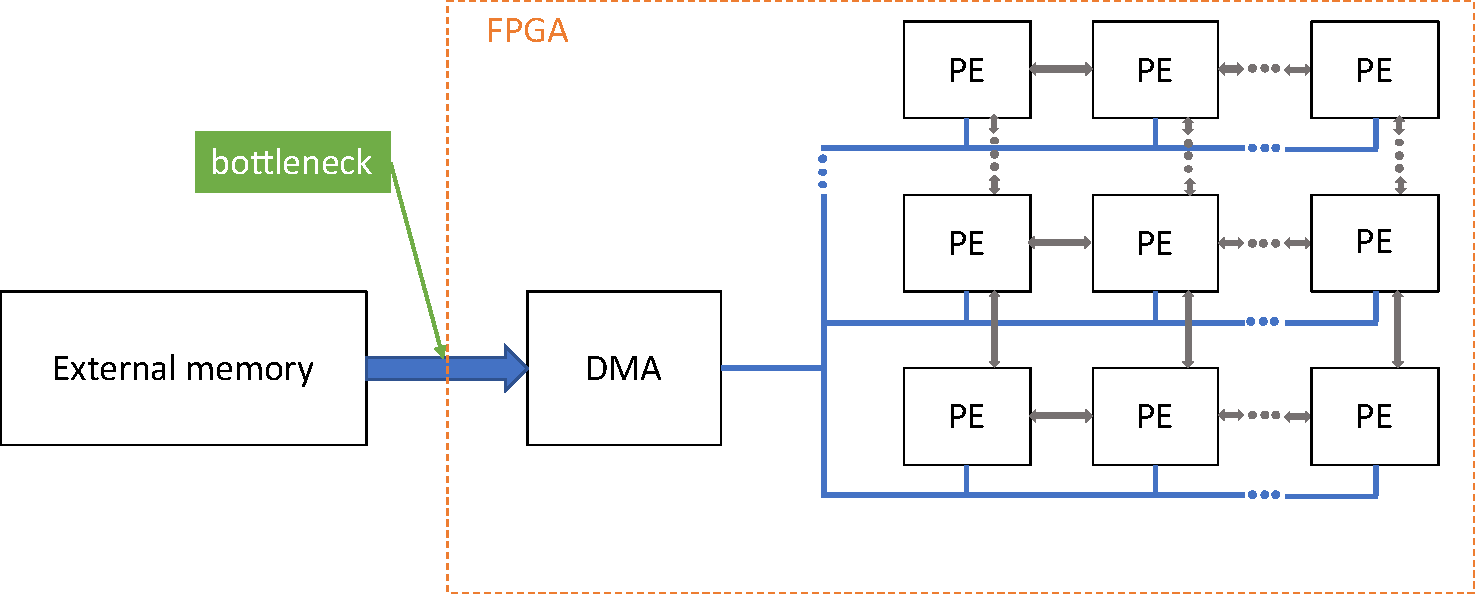
\includegraphics[width=\textwidth]{systArray.pdf}
    \caption{Static Systolic Arrays, inspired by \cite{abdelouahab_accelerating_2018}}
    \label{fig:sytar}
\end{figure}

However, Systolic Arrays have inefficiency problems. First, when the kernel size is much smaller than the maximal kernel size ($K_* << K_m$), there is an underutilization of the resources. For example, \cite{gokhale_240_2014} notes that for $3 \times 3$ kernels, only $9\%$ of the \acrfull{dsp} blocks are used. Second, data caching is not implemented. It means that it has always to fetch input from the external memory and it increases latency \cite{abdelouahab_accelerating_2018, wei_automated_2017}. The device performance is depending then on the memory bandwidth and it becomes memory-bounded. Furthermore, it is not energy efficient. According to \textcite{horowitz_11_2014}, the DRAM accesses severely impact both throughput and energy efficiency. External memory accesses are more expensive by several orders of magnitude in terms of energy and latency.
%
%
\subsubsection{Data-flow MoC for CNNs (2D mapping)}
%
%
Data-flow \acrfull{moc} can be used to accelerate \acrshort{cnn}s on \acrshort{fpga}. This approach is motivated by the feed-forward aspect of the inference stage of \acrshort{cnn}, which is purely data-driven \cite{abdelouahab_accelerating_2018}. Data-flow \acrfull{moc} was firstly investigated by \textcite{lin_li_low_2016}. \acrshort{cnn} can be represented as a graph where:
\begin{itemize}
    \item \textbf{Nodes} are processing units called \textit{actors}. Each actor follows a data-driven execution where the execution is triggered by the availability of input, which is the case for a \acrshort{cnn}.
    \item \textbf{Edges} are communication \acrshort{fifo} channels. Actors exchange data called \textit{tokens} through those \acrshort{fifo} channels.
\end{itemize}
A representation of such a network can be found in Figure \ref{fig:moc}, where $FM_{*}^{i}$ is the ith layer of the \acrshort{fm}.
%
\begin{figure}[H]
    \centering
    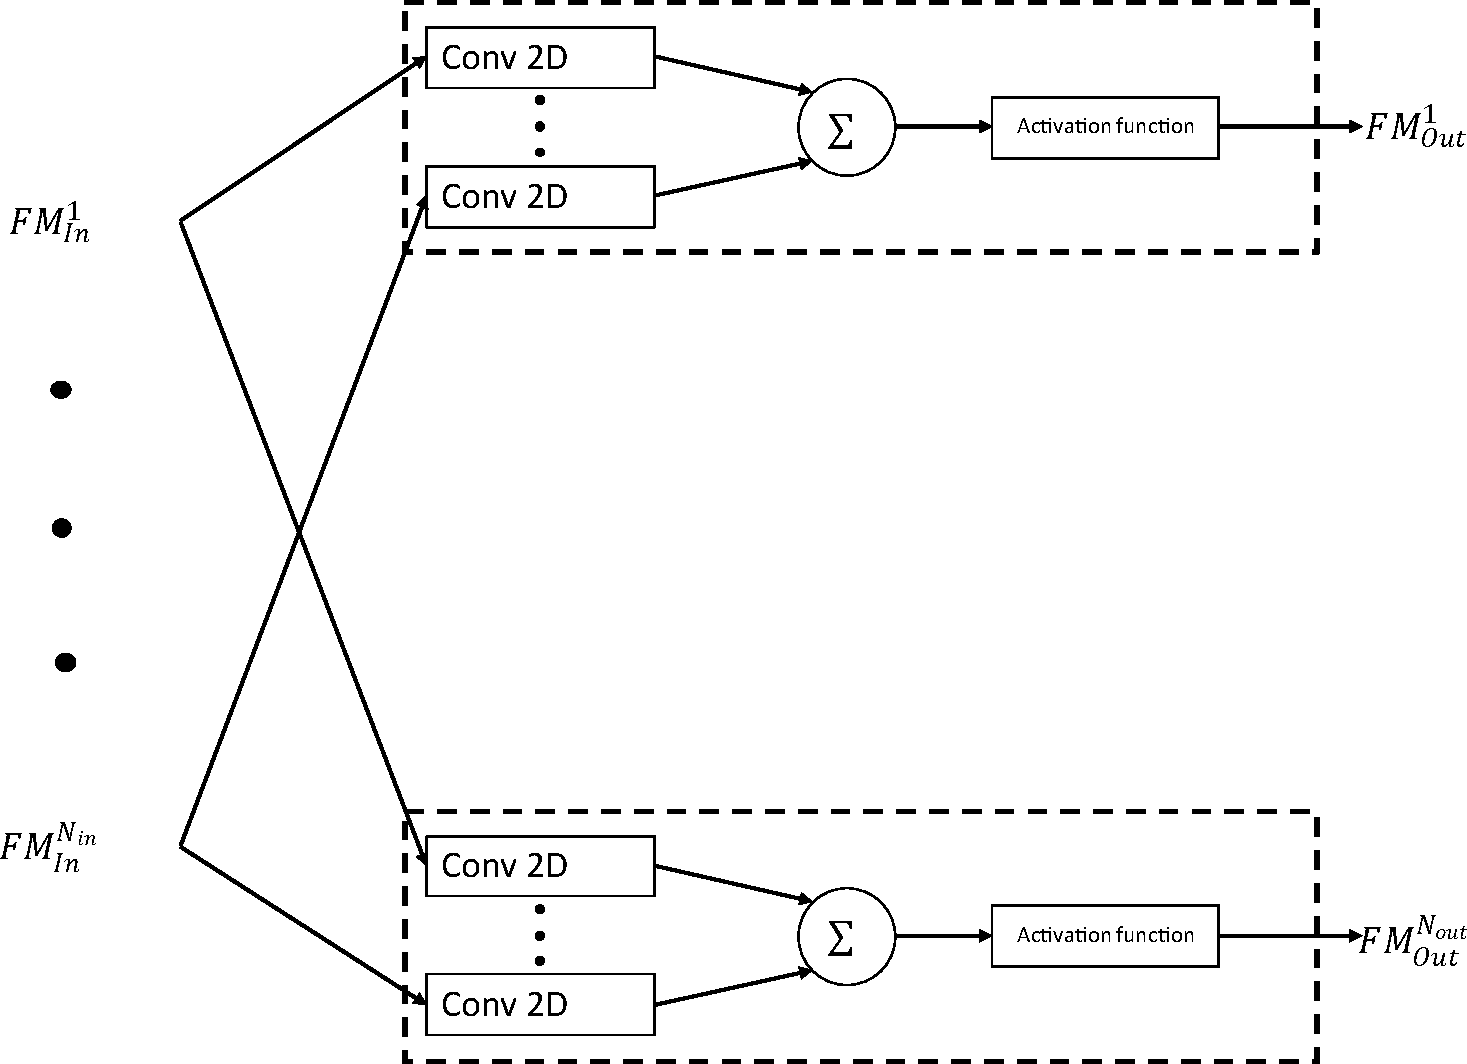
\includegraphics[width=0.6\textwidth]{Moc.pdf}
    \caption{Graph representation of a convolution layer, inspired by \cite{abdelouahab_accelerating_2018}}
    \label{fig:moc}
\end{figure}

As the number of tokens produced and consumed by an actor can be specified in a \acrshort{cnn}, we can apply a static data-flow \cite{lee_static_1987}. Therefore the \acrshort{cnn} can be modeled as a topology matrix and we only need to optimize those matrix components to minimize latency or energy consumption \cite{venieris_latency-driven_2017}. Those parameters are then used to derive \acrshort{pe} and buffer configurations. However, as pointed by \textcite{abdelouahab_tactics_2017}, we need to have direct hardware mapping between the graph and the \acrshort{fpga} to be efficient. It means that all the computations must be unrolled. However, we are then bounded by the hardware resources and the size of \acrshort{cnn}, preventing implementing this approach for deep models \cite{abdelouahab_accelerating_2018}.
%
\subsubsection{Loop Optimizations} \label{subsec:loopopti}
%
%
To overcome the inefficiencies of Systolic arrays and because Data-flow \acrshort{moc} can only be applied to small networks, data must first be cached into the on-chip memory of the \acrshort{fpga} before processing. However, according to \textcite{ma_optimizing_2018}, the on-chip memory of \acrshort{fpga} is not large enough to store all the data (requiring gigabytes). As a result, we need \textit{tiling} to fit a smaller portion of data into memory on-chip \cite{zhang_optimizing_2015}. We can summarize the dataflow as follow: the \acrshort{fpga} fetches a tile of data from external memory to on-chip buffers. Then the data is fed to the \acrshort{pe}s to compute the convolution. The results of the computation are transferred back to on-chip buffers and afterward, to the external memory. When the results are written back to memory, we can fetch a new tile of data. We can see the process in Figure \ref{fig:hierarchy}
%
\begin{figure}[H]
    \centering
    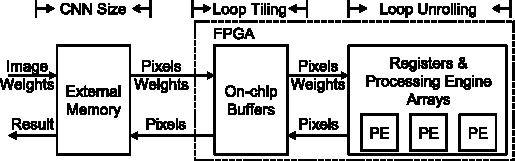
\includegraphics[width=0.75\textwidth]{memhiera.pdf}
    \caption{\acrshort{fpga} memory hierarchy, from \cite{ma_optimizing_2018}}
    \label{fig:hierarchy}
\end{figure}

Consequently, we can define a storage hierarchy with different energy costs. We can define the memory levels as \cite{sze_efficient_2017, horowitz_11_2014}:
%
\begin{enumerate}
    \item \textbf{External Memory}: it stores all the \acrshort{cnn} data. It has a large memory capacity (\textasciitilde GB) but accesses are costly in terms of energy and latency.
    \item \textbf{On-chip memory}: it stores the data fetched from external memory to feed the registers and \acrshort{pe}s. Accesses are less expensive to the external memory but it has less storage (\textasciitilde hundreds of KB).
    \item \textbf{Register}: is associated with the \acrshort{pe}s. The storage capacity is less than a few KB but it is faster and more energy-efficient. Accesses are 1 or 2 orders of magnitude lower energy than from External memory.
\end{enumerate}

Therefore, after tiling, the convolution operation can be decomposed in multiple loops, as observed in Figure \ref{fig:looptiling}. Nevertheless, an improper loop tiling may degrade the performance of the \acrshort{fpga} because we must minimize access to expensive memory levels. The major challenge when implementing a \acrshort{cnn} on \acrshort{fpga} is then to maximize data reuse in small cost memories. To address those problems, loop optimization techniques are applied to the nested loops in Figure \ref{fig:looptiling}. There are three techniques:
%
\begin{enumerate}
    \item \textbf{Loop tiling}: as said above, the on-chip memory of the \acrshort{fpga} is not large enough to store all the weights and \acrshort{fm}s of all \acrshort{cnn} layers \cite{abdelouahab_accelerating_2018}. The \acrshort{fpga} stores a tile of the data, accessed from the external memory, and the lower bound is set on the required on-chip buffer size. The tiling parameters represent the tile size. They are defined as $T_{*}$, where $*$ is the name of the dimension. For example, the size of an input pixel buffer (resp. output) is $T_{ix} \times T_{iy} \times T_{if} \times $ pixel\_datawith ( $ T_{ox} \times T_{oy} \times T_{of} \times $ pixel\_datawith). Furthermore, we have the following constraint: $T_{*} \leq N_{*}$.
    \item \textbf{Loop interchange}: it defines the order of sequential computation of the convolution loops. There are 2 types of loop interchange: \textit{intratile}, patterns of data movements from on-chip memory to registers (loop one to four in Figure \ref{fig:looptiling}); \textit{intertile}, patterns of data movements from external memory to on-chip buffers (the other loops).
    \item \textbf{Loop unrolling}: it determines the number of parallel computations. Four types of unrolling configuration can be done (depending on the loop to unroll). The different configurations can be seen in Figure \ref{fog:unroll}. As the \acrshort{fpga} has constrained resources, it is not always possible to fully unroll a loop. The unrolling parameters are defined as: $P_{*}$, where $*$ is the name of the dimension. We also have the following constraint: $P_{*} \leq T_{*} \leq N{*}$.
\end{enumerate}
%
\begin{figure}[H]
\centering
\begin{lstlisting}[language=Java]
for (int of=0;of<N;of+=Tof){
  for (int iy=0;iy<Niy,iy+=Tiy){
    for (int ix=0;ix<Nix,ix+=Tix){
      for (int if=0;n<C;if+=Tif){
        // DRAM: Load in on chip buffers the tiles
        // X[l,if:if+Tif,iy:iy+Ty,ix:ix+Tix]
        // Theta [l,n:n+Tof,if:if+Tif,j,k]
          for (int tof=0;tof<Tof;tof++){ -> Loop-4
            for (int tiy=0;tiy<Tiy,tiy++){ -> Loop-3
              for (int tix=0;tix<Tix,tix++){ -> Loop-3
                for (int tif=0;tof<Tif;tif++){ -> Loop-2
                  for (int ky=0;ky<Nky,ky++){ -> Loop-1
                    for (int kx=0;kx<Nkx,kx++){ -> Loop-1
                      Y[tof,tiy,tix] += X[tif,tiy+ky,tix+kx] *
                      W[tof,tif,ky,kx];
          }}}}}}
          // DRAM: Store output tile
}}}}
    \end{lstlisting}
    \caption{Loop Tiling, from \cite{abdelouahab_accelerating_2018}}
    \label{fig:looptiling}
\end{figure}
%
\begin{figure}[H]
    \centering
    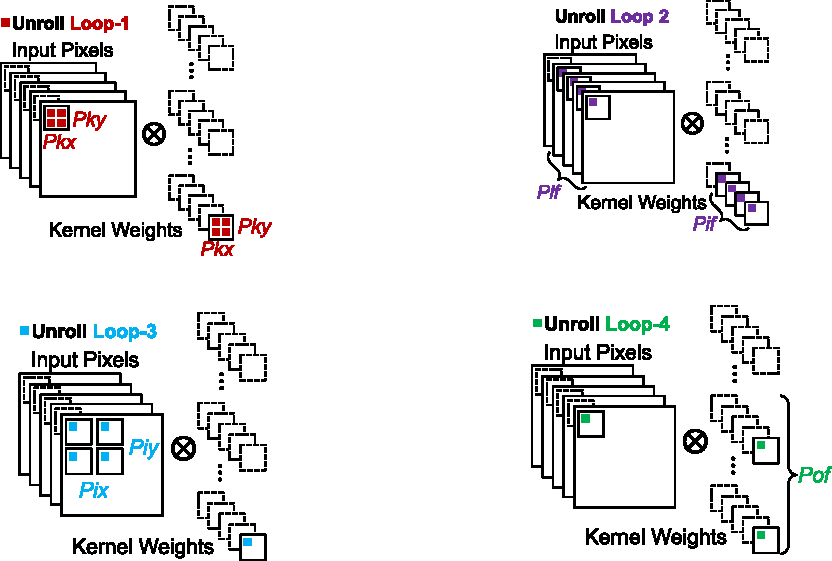
\includegraphics[width=\textwidth]{unroll.pdf}
    \caption{Loop unrolling configurations, from \cite{ma_optimizing_2018}}
    \label{fog:unroll}
\end{figure}

The loop optimization design variables determine the number of \acrshort{pe}s (unrolling parameters), the buffer size, and the number of external memory access (tiling parameters). We are going to review different studies of the design space exploration of unrolling parameters, tiling parameters, and loop interchange, to design the most efficient accelerator on the target platform.

The work of \textcite{zhang_optimizing_2015} proposes an analytical solution using the roofline model \cite{williams_roofline_2009} to identify the CNN design with the best performance and lowest \acrshort{fpga} resource requirement. They chose a loop unrolling of ($T_{if} \times T_{of}$) to avoid complex connection topologies for all arrays. It allows spatial reuse of pixels for $T_{of}$ unrolls, and the temporal reuse of weight for ($T_{ox} \times T_{oy}$). However, the disadvantage of this method is the need for a large local memory to store the partial sums ($T_{of} \times T_{ox} \times T_{oy}$).

Once the loop ordering and unrolling parameters have been set, the roofline model can be used to find the optimal tiling parameters. \textcite{mittal_survey_2020} defines this design space exploration method as: \textquote{\textit{The roofline model relates performance to computational performance and off-chip memory traffic}}. As an implementation can either be computation-bounded or memory-bounded, it uses those two limits to find the best trade-off between memory bandwidth and computational speed, where $CTC$ is the communication-to-communication ratio.
\begin{enumerate}
    \item \textbf{Computational roof}: $= \frac{\text{\# \ of \ operations}}{\# \ of \ execution \ cycles}$.
    \item \textbf{CTC ratio}: $= \frac{\text{\# \ of \ operations}}{\# \ of \ external \ data \ access}$
\end{enumerate}
Therefore, the achievable performance can be computed using equation \ref{eq:atperf}.
\begin{equation}
Att \ perf = min \ (Computational \ roof; CTC \ ratio \times bandwidth)
\label{eq:atperf}
\end{equation}

The roofline method is shown in Figure \ref{fig:roofmeth}. We can conclude that the best solution to pick is solution C since it offers the best performance while requiring the least bandwidth \cite{zhang_optimizing_2015}.
%
\begin{figure}[H]
    \centering
    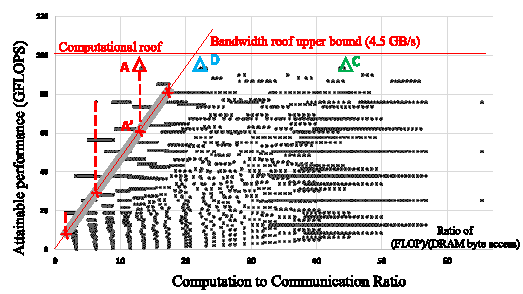
\includegraphics[width=\textwidth]{roofmethod.pdf}
    \caption{Design space of platform-supported designs, from \cite{zhang_optimizing_2015}}
    \label{fig:roofmeth}
\end{figure}

\textcite{motamedi_placid_2017} chose the best parameters according to the resources and the best data reuse scheme of the target platform. They did not tile on the kernel on the spatial axis because recent \acrshort{cnn}s have small filters and it would mean that a pixel can be loaded multiple times. As the tile goes over the input and output \acrshort{fm} channel, there is a choice between maximizing the reuse of the input \acrshort{fm} (MIR, each \acrshort{fm} is loaded once but some intermediate results have to be written back to memory) or output \acrshort{fm} (MOR, to avoid writing back intermediate results to memory but some input \acrshort{fm} have to be loaded more than once). Then they performed an exhaustive search on the tiling and \acrshort{pe} parameters to find the optimal design. It can be layer-specific (but the \acrshort{fpga} needs dynamic reconfiguration and \textcite{zhang_optimizing_2015} proved that it is inefficient) or values are fixed for all layers.

A different approach, studied by \textcite{ma_optimizing_2018}, proposes a design space exploration regarding various design objectives:
\begin{itemize}
    \item \textbf{Latency}: $P_*$ should be common factors of  $T_*$ for all convolution layers to fully utilize \acrshort{pe}s and $T_*$ should be the common factors of  $N_*$ to make full use of external memory transactions.
    \item \textbf{Partial sum storage}: to minimize the concurrent storage of partial sums in local memory and allowing to keep them into the PE, we should promote the computation of an output pixel to evacuate it to the external memory.
    \item \textbf{On-chip memory access}: on-chip memory access can be minimized by reusing at most pixels or weights in the \acrshort{pe}s.
    \item \textbf{External memory access}: to minimize external access, a sufficient buffer size should be assigned to pixels and weights.
\end{itemize}

They proposed two flowcharts in Figure \ref{fig:flowchart} to determine the number of partial sums and external accesses. 
%
\begin{figure}[H]
\centering
    \begin{subfigure}{.45\textwidth}
    \centering
    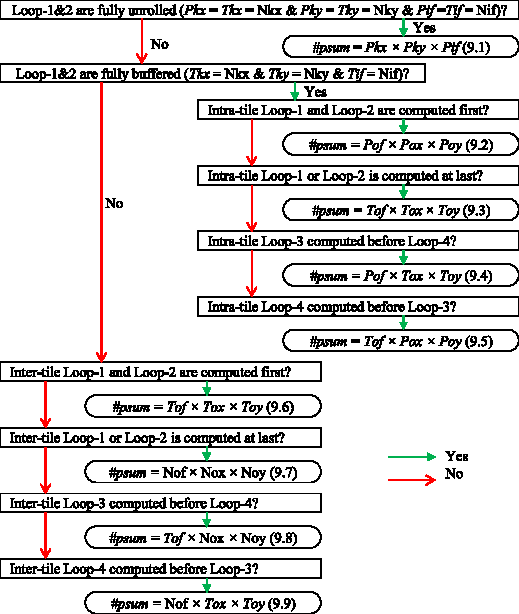
\includegraphics[width=\linewidth]{fwch1.pdf}
    \caption{ }
    \end{subfigure}
    \begin{subfigure}{.45\textwidth}
    \centering
    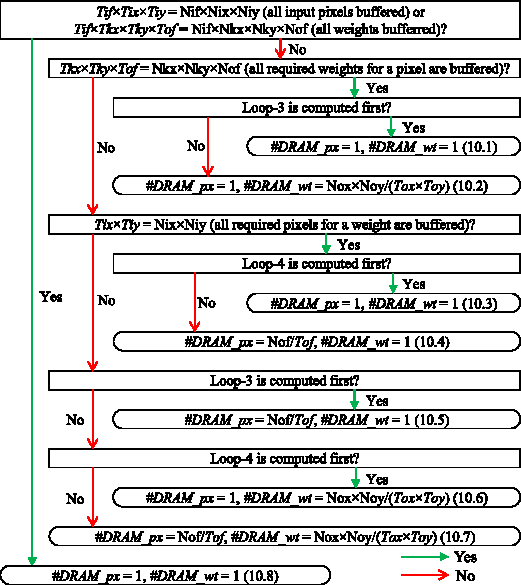
\includegraphics[width=\linewidth]{fwch2.pdf}
    \caption{ }
    \end{subfigure}
    \caption{Design space exploration of: (a) total number of partial sums that need to be stored in memory; (b) the number of external memory accesses, from \cite{ma_optimizing_2018}}
    \label{fig:flowchart}
\end{figure}

%%%%%%%%%%%%
\subsection{Model Optimizations} \label{subsec:mdopti}
As mentioned previously, the major issues, when implementing a \acrshort{cnn} on an \acrshort{fpga}, are the \acrshort{cnn} size and its computational complexity. Research was done to develop techniques tackling those two issues by directly modifying the \acrshort{cnn} architecture. \textcite{nurvitadhi_can_2017} believe that sparsity exploitation and extremely compact data types will become the norm in next-generation \acrshort{cnn}s.
%
%
\subsubsection{Efficient Model Design}
%
Section \ref{subsec:models} presented several state-of-the-art models. However, those models (except MobileNetV2) were designed to provide the highest performance possible but did not consider the implementation of such models on mobile and embedded devices \cite{iandola_squeezenet_2016}. Therefore, several other models were designed to run on such constrained platforms trading a reduction of the number of parameters and operations in exchange for a drop of accuracy. Indeed, if we observe Figure \ref{fig:archi}, the lightweight models do not match the high-performance ones in terms of accuracy only.

A clever choice of design decreases the number of parameters and computations of the model while reducing the drop of accuracy. As many approaches were proposed to reduce the size of a model, this study will focus on architectures that target the embedded space. This section describes five of these architectures:
\begin{itemize}
    \item \textbf{SqueezeNet} \cite{iandola_squeezenet_2016} was focused on reducing the number of parameters of AlexNet (see Section \ref{subsec:models}) by introducing a new building block: \textbf{Fire Module}. Therefore, their architectures are very similar. SqueezeNet replaces all layers (except the first and last one) by \textbf{Fire Modules}. The \textbf{Fire Module}, observed in Figure \ref{fig:archi_building_block:sqn}, is composed of two convolutional layers. The first one called \textit{squeeze block} only performs $1 \times 1$ convolutions to squeeze the number of input channels. The reduction of the number of channels decreases the computational complexity and number of parameters of the next convolutional layer. Moreover, they also chose $1 \times 1$ convolution because it requires fewer parameters than $3 \times 3$ convolution.
    The second convolutional layer called \textit{expand block} is composed of $1 \times 1$ and $3 \times 3$ convolutions. With this architecture, the size of AlexNet is decreased from $240$MB to $4.8$MB \cite{iandola_squeezenet_2016}. It can even be reduced to $0.47$MB without a drop in accuracy method by applying Deep Compression \cite{han_deep_2016}. However, it has a big memory footprint, is slower in runtime, and consumes more energy than AlexNet \cite{sze_efficient_2017}.
    %
    \item \textbf{MobileNet} \cite{howard_mobilenets_2017} uses \acrshort{dsc}, described in Section \ref{subs:dsc}, to build small and low latency models that can fulfill the design requirements, as can be seen in Figure \ref{fig:archi_building_block:mbn}. Two hyper-parameters are used to set the model size and throughput:
    %
    \begin{itemize}
        \item The width multiplier $\alpha \in [1; 0[$, which reduces the number of input and output channels at each layer,
        \item The resolution multiplier $\rho \in [1; 0[$,  which reduces spatially the input and output \acrshort{fm}s at each layer.
    \end{itemize}
    %
    \item \textbf{ShuffleNet}  was developed by \textcite{zhang_shufflenet_2018}, in 2018. It is designed to be a computation efficient architecture, especially for mobile devices with very limited computing power. Indeed, it reduces the computation cost while maintaining the accuracy by using \textbf{pointwise group convolution}, decreasing the computation complexity of $1 \times 1$ convolutions. It also uses \textbf{channel shuffle} operation on the channels such that \textbf{group convolutions} obtain information from different groups. Then more powerful structures can be built with multiple group convolutional layers. However, the group convolutions and the bottleneck structures add \acrfull{mac} which is a non-negligible cost \cite{ma_shufflenet_2018}. The group convolution contributes to network fragmentation and reduces parallelism. Moreover, the \textquote{Add} operation, as seen in Figure \ref{fig:archi_building_block:shn}, is quite significant.
    %,
    \item \textbf{NasNet} was developed by \textcite{zoph_learning_2018}, in 2018. The idea was to use a search method called \acrfull{nas}, to find good convolutional architectures on a specific dataset. For that purpose, NasNet uses a \acrfull{rnn} to generate efficient architectures. The \acrshort{rnn} generates sample child networks with different architectures, which are trained to convergence. The accuracy of the child networks is used to train the \acrshort{rnn}, which will generate better architectures over time. A convolution layer can be seen in Figure \ref{fig:archi_building_block:nasn}. The learned architecture is flexible as it may be scaled in terms of computational cost. The network provides a higher accuracy with comparable parameters and \acrshort{mac} than MobileNet and ShuffleNet (described previously) \cite{zoph_learning_2018}. However, the resulting network ends up very complex \cite{sandler_mobilenetv2_2018}.
    %
    \item \textbf{MobileNetV2} was developed by \textcite{sandler_mobilenetv2_2018}, in 2018. It is an improvement of MobileNet (described previously) in terms of accuracy and does not require special operators. It has also a smaller memory footprint. Furthermore, MobileNetV2 has faster inference and fewer parameters than MobileNet. MobileNetV2 has already been explained in Section \ref{subs:mbv2}.
\end{itemize}
%
\begin{figure}[H]
    \centering
    %
    \begin{subfigure}[t]{0.49\linewidth}
        \centering
        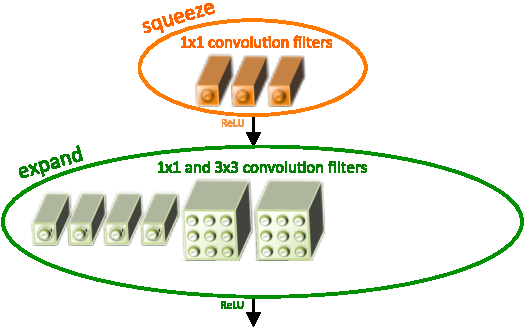
\includegraphics[width=\textwidth, height=0.3\textheight, keepaspectratio]{squeeze.pdf}
        \caption{Squeezenet Fire Module\cite{iandola_squeezenet_2016}}
        \label{fig:archi_building_block:sqn}
    \end{subfigure}
    %
    \begin{subfigure}[t]{0.49\linewidth}
        \centering
        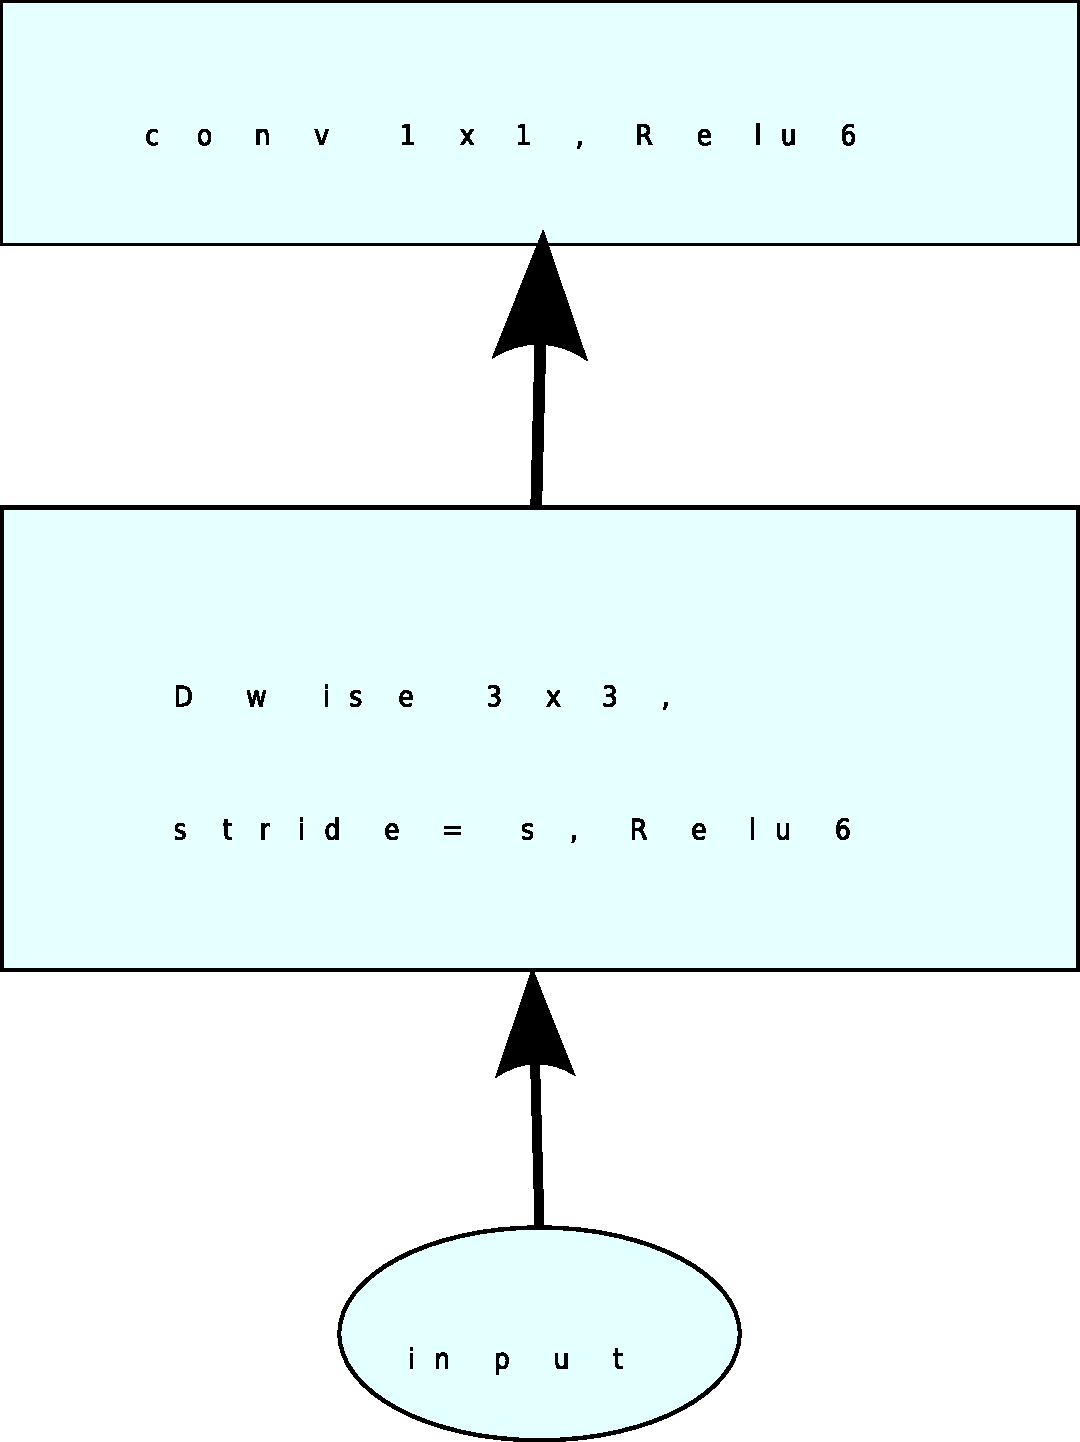
\includegraphics[width=\textwidth, height=0.2\textheight, keepaspectratio]{mobilenet.pdf}
        \caption{MobileNet convolutional block \cite{howard_mobilenets_2017}}
        \label{fig:archi_building_block:mbn}
    \end{subfigure}
    %
    \begin{subfigure}[t]{0.49\linewidth}
        \centering
        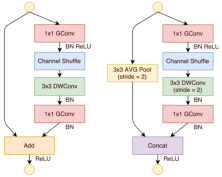
\includegraphics[width=\textwidth, height=0.2\textheight, keepaspectratio]{shufflenet.pdf}
        \caption{ShuffleNet convolutional block \cite{zhang_shufflenet_2018}}
        \label{fig:archi_building_block:shn}
    \end{subfigure}
    %
    \begin{subfigure}[t]{0.49\linewidth}
        \centering
        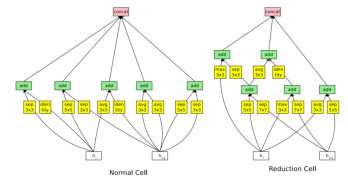
\includegraphics[width=\textwidth, height=0.3\textheight, keepaspectratio]{nasnet.pdf}
        \caption{NasNet convolutional blocks \cite{zoph_learning_2018}}
        \label{fig:archi_building_block:nasn}
    \end{subfigure}
    %
    \begin{subfigure}[t]{0.49\linewidth}
        \centering
        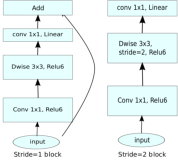
\includegraphics[width=\textwidth, height=0.2\textheight, keepaspectratio]{mobilenet2.pdf}
        \caption{MobileNetv2 convolutional blocks \cite{sandler_mobilenetv2_2018}}
        \label{fig:archi_building_block:mb2n}
    \end{subfigure}
    %
    \caption{Convolutional block from different architectures}
    \label{fig:archi_building_block}
\end{figure}

The architecture used in this work was developed to implement MobileNetV2 because of its simplicity and its state-of-the-art performance (see Table \ref{tab:mbv2}). Moreover, MobileNetV2 requires fewer parameters while providing state-of-the-art accuracy when comparing to the different architectures, as shown in Figure \ref{fig:archi}.
%
\begin{table}[H]
    \center
    \begin{tabular}{ | c | c | c c | c| }
        \hline \hline
        Network & Top 1 & Params & MAdds & CPU \\
        \hline \hline
        MobileNetV1 & 70.6 & 4.2M & 575M & 113ms \\
        ShuffleNet (1.5) & 71.5 & \textbf{3.4M} & 292M & - \\
        ShuffleNet (x2)  & 73.7 & 5.4M & 524M & - \\
        NasNet-A & 74.0 & 5.3M & 564M & 183ms \\
        \hline
        MobileNetV2 & \textbf{72.0} & \textbf{3.4M} & \textbf{300M} & \textbf{75ms} \\
        MobileNetV2 (1.4) & \textbf{74.7} & 6.9M & 585M & \textbf{143ms} \\
        \hline \hline
    \end{tabular}
    \caption{Performance on ImageNet, comparison for different networks \cite{sandler_mobilenetv2_2018}}
    \label{tab:mbv2}
\end{table}

\begin{figure}[H]
    \centering
    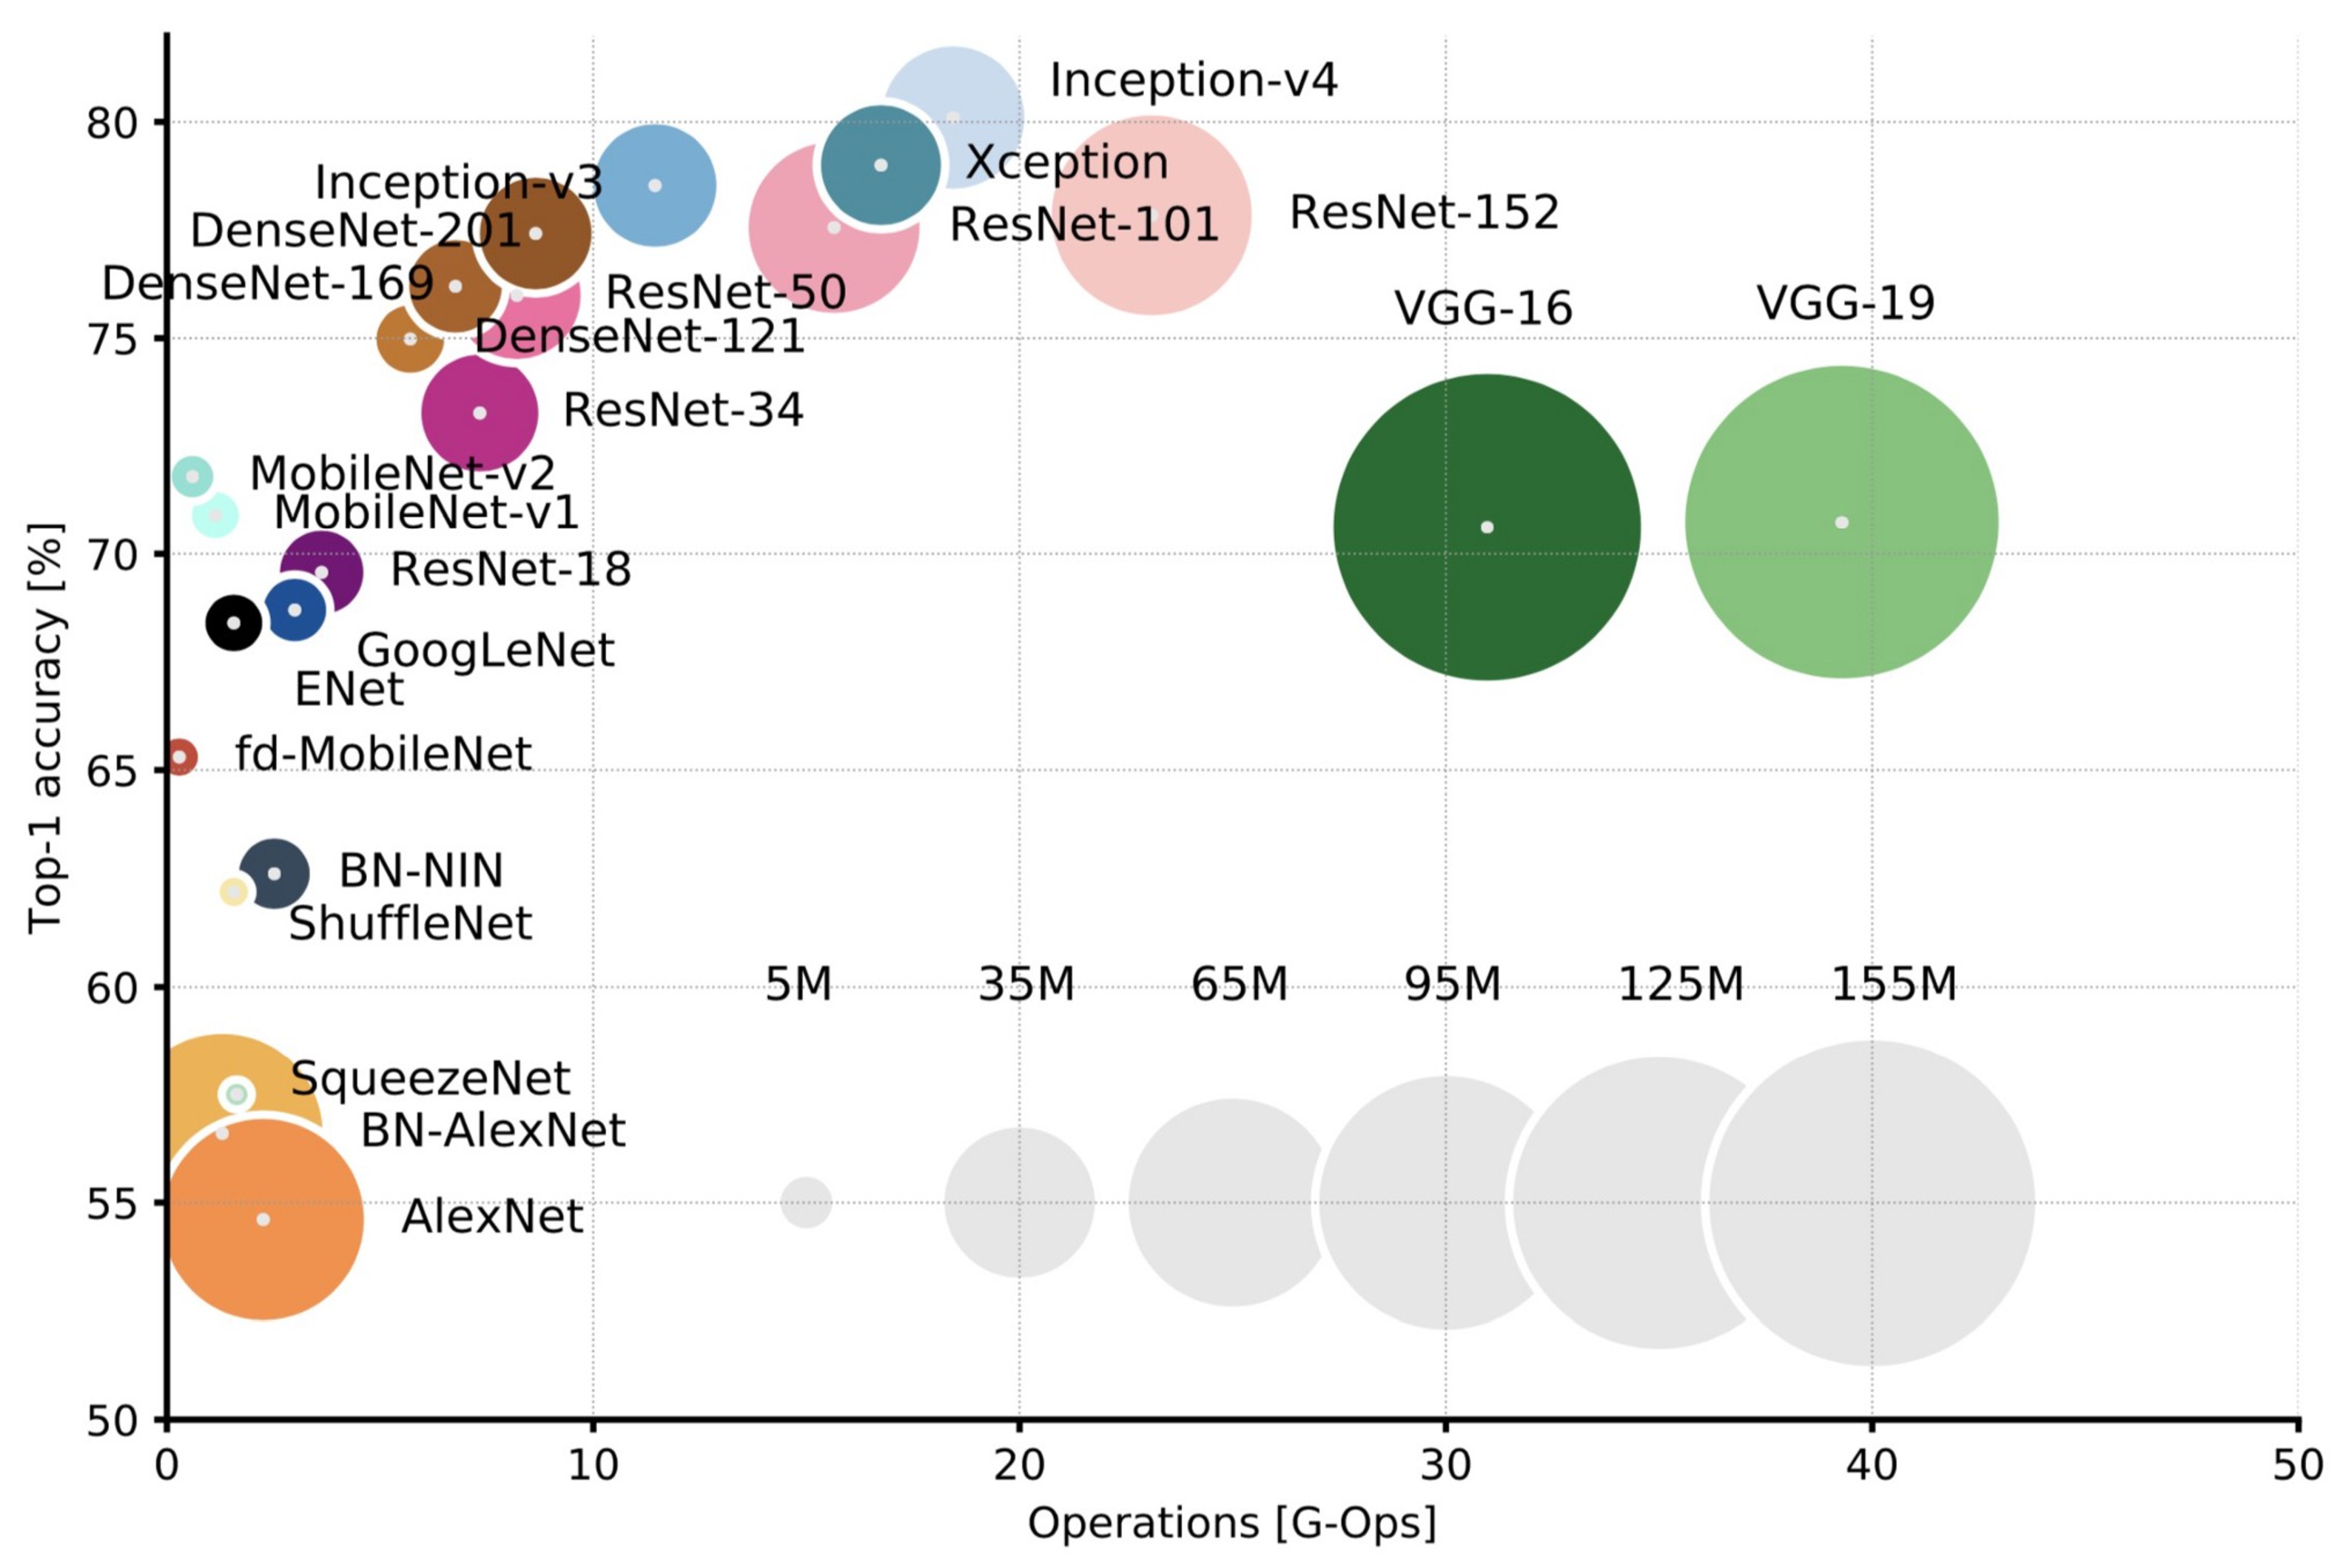
\includegraphics[width=0.9\textwidth]{archi.pdf}
    \caption{Ball chart reporting the Top-1 accuracy of various architectures vs. their computational complexity \cite{canziani_analysis_2017}}
    \label{fig:archi}
\end{figure}
%
\subsubsection{Pruning} \label{subs:pruning}
%
To improve the inference phase of a \acrshort{cnn}, pruning can be used, especially for platforms with limited computational resources \cite{liu_rethinking_2019}. According to \textcite{liu_rethinking_2019, denton_exploiting_2014}, the huge number of parameters in a network might create a problem of \textbf{over-parametrization}. Over-parametrization means that there are redundancies in \acrshort{nn} parameters and that the same performance could be achieved with only a subset of them. In other words, a lot of parameters are unimportant or unnecessary \cite{cheng_recent_2018}. Pruning is defined as removing the parameters considered as not important. For example, \textcite{baoyuan_liu_sparse_2015} achieve more than 90\% sparsity of parameters in convolutional layers in AlexNet with less than 1\% accuracy loss.

We can explain why pruning works by \textbf{The Lottery Ticket Hypothesis} \cite{frankle_lottery_2018, frankle_early_2020}: \textquote{\textit{A randomly initialized, dense neural network contains a subnetwork that is initialized such that—when trained in isolation—it can match the test accuracy of the original network after training for at most the same number of iterations.}} From this postulate, those unimportant weights can be set to zero (prune) because they do not improve the accuracy of the model.

According to \textcite{cheng_recent_2018}, pruning has two major benefits for the inference phase. First, less storage is required. Indeed, the non-pruned weights are sparsely distributed among the kernels. Thus, they can be stored in a compressed format reducing memory utilization. Second, pruning reduces the arithmetic complexity of the network. As convolutions perform a weighted sum with the input \acrshort{fm}, each \acrfull{mac} operation with a pruned weight can be discarded. Moreover, \textcite{han_learning_2015, mao_exploring_2017, kang_accelerator-aware_2020} pointed out that some pruning ratios can also improve the accuracy of the network, which can be explained by a form of regularization.

Various pruning schemes are focused on increasing the sparsity of the network without a drop of accuracy \cite{han_deep_2016, han_learning_2015}.  We call this pruning scheme where all unimportant parameters are pruned without extra constraint \textbf{unstructured pruning} \cite{cheng_recent_2018}. However, it is challenging to exploit the performance and the high parallelism of \acrshort{fpga} with this kind of pruned network. Indeed, this kind of pruning scheme creates irregularities in the data access pattern \cite{zhu_efficient_2020}. It means that the number of pruned weights is different in each kernel, and we should adapt the circuitry to the worst case. As a consequence, all filters conduct wasteful operations except the worst case \cite{shimoda_filter-wise_2019}. Furthermore, \textcite{anwar_structured_2017} pointed out that unstructured pruning requires overhead for computing addresses of the sparse non-pruned elements. Therefore, we should find pruning patterns that would be more hardware-friendly.

In contrast to the unstructured pruning, we have \textbf{structured pruning} schemes \cite{kang_accelerator-aware_2020}. They combine a structure regularization for accuracy and locality optimization for computation efficiency. According to \textcite{anwar_structured_2017}, \textquote{\textit{Structured pruning has no or little extra costs}}. We can categorize the various schemes into different groups \cite{cheng_recent_2018, kang_accelerator-aware_2020, anwar_structured_2017, wen_learning_2016}:
\begin{itemize}
    \item \textbf{Depth-wise}: all the weights of a layer are pruned. The layer is then removed.
    \item \textbf{Kernel-wise}: instead of pruning all the weights, we keep a ratio of kernels, which means a reduction of the number of output channels. This pruning scheme is provided in Figure \ref{fig:struct_pruning:fw}.
    \item \textbf{Channel-wise}: it is one of the most popular methods because it still can fit in the convolutional deep learning frameworks \cite{liu_rethinking_2019}. A layer of the input \acrshort{fm} is pruned, which means that the layer is also pruned in all the kernels, as can be seen in Figure \ref{fig:struct_pruning:chw}.
    \item \textbf{Shape-wise}: we prune the same weights in each kernel or group of kernels. For example, this pruning scheme was used in \textcite{zhu_efficient_2020}. It is illustrated in Figure \ref{fig:struct_pruning:sw}
\end{itemize}
%
\begin{figure}[H]
    \centering
    %
    \begin{subfigure}[t]{.32\textwidth}
    \centering
    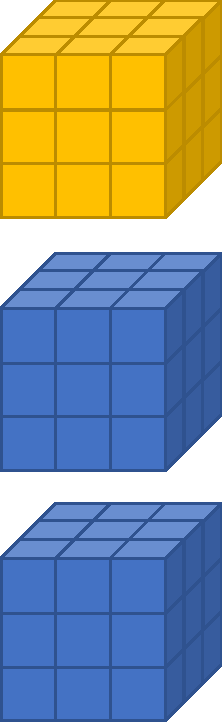
\includegraphics[width=0.33\linewidth]{filterwise.pdf}
    \caption{kernel-wise pruning}
    \label{fig:struct_pruning:fw}
    \end{subfigure}
    %
    \begin{subfigure}[t]{.32\textwidth}
    \centering
    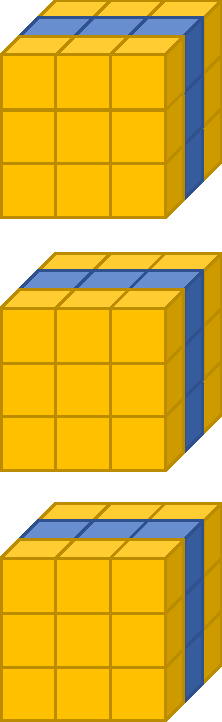
\includegraphics[width=0.33\linewidth]{channelwise.pdf}
    \caption{channel-wise pruning}
    \label{fig:struct_pruning:chw}
    \end{subfigure}
    %
    \begin{subfigure}[t]{.32\textwidth}
    \centering
    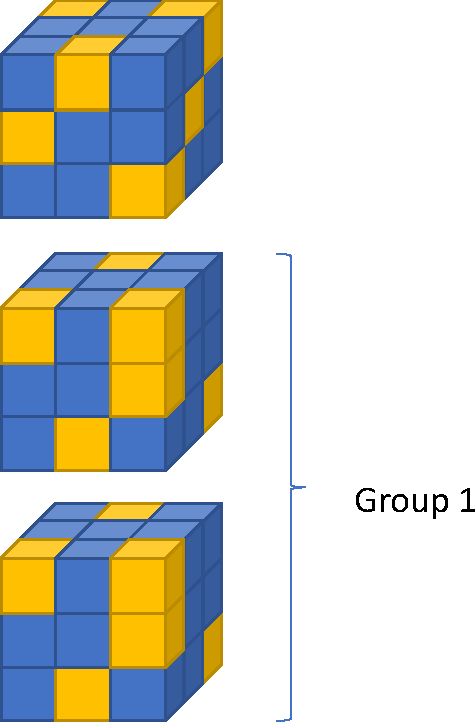
\includegraphics[width=0.70\linewidth]{shapewise.pdf}
    \caption{shape-wise pruning}
    \label{fig:struct_pruning:sw}
    \end{subfigure}
    %
    \caption{Structured pruning schemes, where the yellow weights are the pruned ones, inspired by \cite{cheng_recent_2018}}
    \label{fig:struct_pruning}
\end{figure}
%
The previously cited pruning schemes are ordered from very coarse-grained to fine-grained sparsity \cite{mao_exploring_2017}. As explained previously, coarse-grained sparsity (channel-wise and filter-wise pruning) provides a higher acceleration and can be used when implementing \acrshort{cnn} on \acrshort{gpu} or \acrshort{cpu} \cite{cheng_recent_2018, mao_exploring_2017}. However, finer-grained ones provide higher accuracy and as the sparsity increases, the accuracy is less affected, as can be seen in Figure \ref{fig:pruning-accuracy}. Therefore, this work focuses on developing customized hardware that can exploit a more fine-grained sparsity \cite{mao_exploring_2017} to provide a higher pruning while limiting the drop of accuracy.
%
\begin{figure}[H]
    \centering
    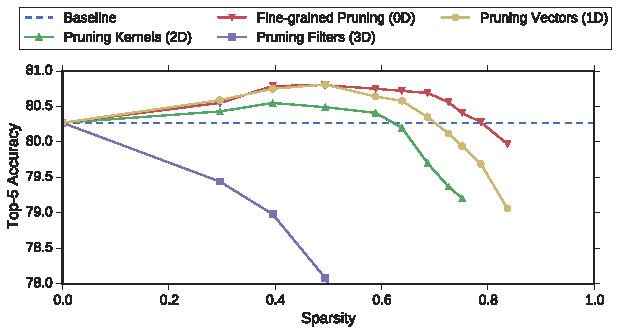
\includegraphics[width=\textwidth]{accuracysparsity.pdf}
    \caption{Accuracy-Sparsity Curve of AlexNet obtained by pruning \cite{mao_exploring_2017}}
    \label{fig:pruning-accuracy}
\end{figure}
%
Some studies focused on the acceleration of the inference step of lightweight models thanks to pruning. \textcite{zhang_channel_2019, tu_pruning_2019} applied pruning on \acrshort{dsc} kernels. They both chose \textbf{Channel-wise} pruning because it does not create sparse connections and it efficiently improves the speed of the inference. It also reduces the computational cost of the $1 \times 1$ (pointwise) convolutions, which has the biggest number of parameters and computational complexity. In MobileNet, it is about 95\%. By discarding one channel, the associated depthwise convolution is also avoided.
Moreover, the pointwise kernel producing that channel in the previous block can also be pruned. We can see the process in Figure \ref{fig:pruning_dsc}.
%
\begin{figure}[H]
    \centering
    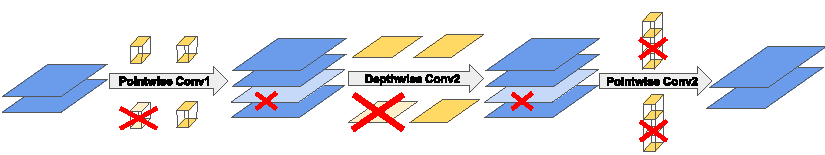
\includegraphics[width=\textwidth]{channelwise_ex.pdf}
    \caption{Pruning a depthwise separable convolution \cite{tu_pruning_2019}}
    \label{fig:pruning_dsc}
\end{figure}

\textbf{In this work, we focus on a structured pruning scheme for depthwise separable convolution. More precisely, we develop an architecture on \acrshort{fpga} than combines both advantages of pruning and depthwise separable convolution.}
%
\subsubsection{Quantization} \label{subs:quantization}
%
%
Quantization is an approach to trade accuracy for a decrease of the storage requirements of a network \cite{han_deep_2016}. Indeed, we can define quantization as the reduction of the number of bits representing a weight or pixel. Moreover, instead of using a floating-point number, we can use a \textbf{fixed-point number} \cite{cheng_recent_2018}. As said previously, fixed-point numbers are known to be more efficient on hardware such as \acrshort{fpga} because we can use integer arithmetic \cite{david_hardware_2007}. Quantization to fixed-point numbers can then reduce the memory requirement and the latency of the inference stage.

The format to encode the fixed-point representation of a real number is the \textit{Q-format} \cite{ward_real-time_2001}. A N-bit number, noted $Q_{m.n}$, is divided into two parts separated by an implied binary point. The $m$ bits are used to represent the integer part of the number (including the sign bit), and the $n$ bits are used to represent the fractional part, as can be seen in Figure \ref{fig:Qformat}. The bitwidth associated with each part can be either the same, either fine-tuned for each layer after analysis. Indeed, \textcite{qiu_going_2016, yin_high_2018} choose a different range for each layer, but doing it for every weight is not memory-efficient.
%
\begin{figure}[H]
    \centering
    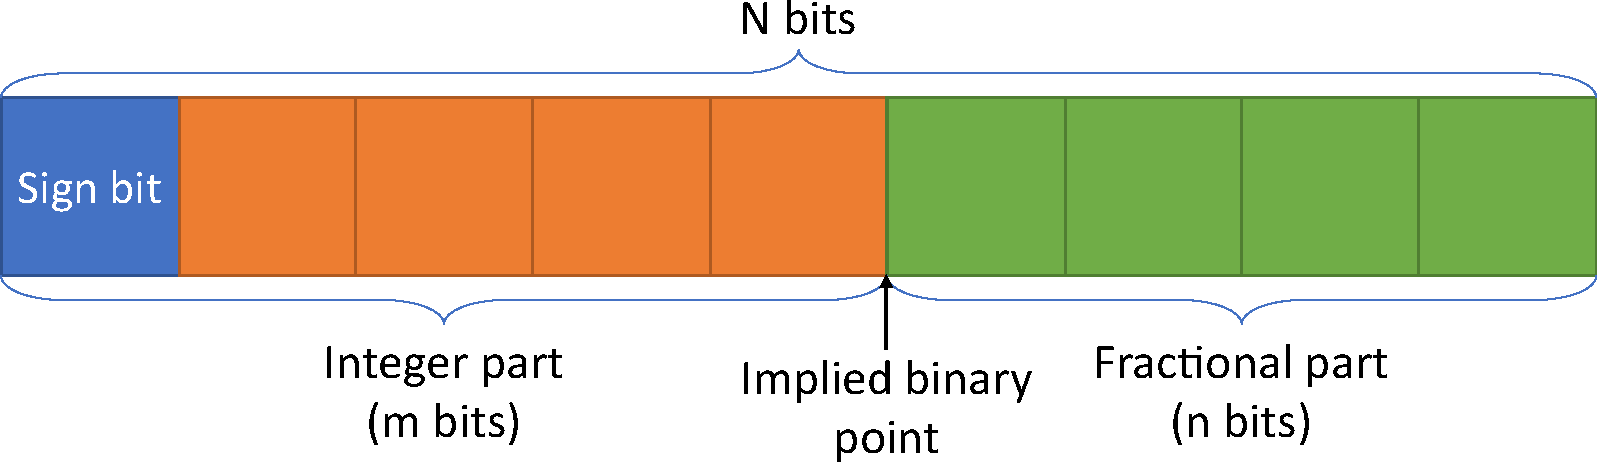
\includegraphics[width=\textwidth]{Qformat.pdf}
    \caption{Illustration of the Q-format}
    \label{fig:Qformat}
\end{figure}

As pointed out by \textcite{han_deep_2016}, quantization and pruning techniques are orthogonal and can be combined to compress further the network. Unfortunately, not all existing networks are friendly for quantization, like MobileNet. MobiletNet with quantized pixels and weights has a large drop of accuracy compared with its Non-quantized version (70.50\% using floating-point model vs 1.80\% using an 8-bit pipeline) \cite{sheng_quantization-friendly_2018}. However, the work of \textcite{sheng_quantization-friendly_2018} showed that the source of the accuracy drop was the design of the separable convolution core layer. They proposed therefore a new quantization-friendly separable convolution core layer. Works on MobileNetV2 should then be done to verify the fixed-point inference accuracy. Still, an 8-bit pipeline might not be optimal for MobilNetV2 as increasing the bitwidth to 16-bit could boost accuracy \cite{cheng_recent_2018}. This bitwidth is also widely used \cite{huimin_li_high_2016, bai_cnn_2018}. 

\textbf{Therefore, 16-bit fixed-point Q-format is adopted for input data, weights, and intermediate data in the frame of this thesis}. \textbf{Moreover, as said previously in Section \ref{subs:acti}, we can limit the integer part to 3 bits (one bit is added to express the sign of the weights), and we can use $Q_{4.12}$.}

%%%%%%%%%%%%
\section{Conclusion} \label{sec:cclopti}
We can observe on table that pruning seem to be a preferable solutions because ... \newline \newline
On next chapter we are going to explore how to handle pruning on \acrshort{fpga}.


%
\fbox{\parbox{ \linewidth \fboxrule \fboxsep }{ \textbf{Conclusion about the background}:

\vspace{5mm}
We have seen in this chapter what is a \acrshort{cnn}, how to build, and train it. We have also seen that the most performing models have a huge computational complexity and memory utilization, which limit the implementation of such models on mobile platforms, such as \acrshort{fpga}. Different approaches can be explored such as fast convolutions algorithms. But they only reduce the computational complexity while increasing hardware utilization. Therefore, pruning and model designs seem to be promising optimizations because they both aim at reducing those problems. Therefore, this work focus on the use of both approaches to see if their gain can be combined. To show our results, we apply pruning on MobileNetV2. As quantizing is an orthogonal approach to pruning, we also use 16-bit fixed-point formats because the loss of accuracy can be controlled.
}}
\afterpage{\blankpage}
\cleardoublepage
\newpage
